\documentclass{article}
\input{../../../LaTex/preamble/preamble_article.tex}


\title{高中物理}
\author{马祥芸}


\begin{document}
\maketitle
\tableofcontents
\zihao{-4}
\newpage

\section{匀变速直线运动问题}

\subsection{中间时刻/平均速度}
中间时刻速度$v_{\frac{t}{2}}$与平均速度$\overline{v}$是同一个值
$$
    v_{\frac{t}{2}} = v_{0} + \frac{at}{2} = \frac{v_{0}}{2} +  (\frac{v_{0}}{2} + \frac{at}{2})   = \frac{v_{0}+v_{t}}{2} = \overline{v}
$$

中间位置速度

\begin{numcases}{}
    \label{1} 2 a\frac{x}{2} = v_{\frac{x}{2}}^{2} - v_{0}^{2}  \\
    \label{2} 2 a\frac{x}{2} = v_{t}^{2} - v_{\frac{x}{2}}^{2}
\end{numcases}

由方程$(1) - (2)$ 得到 $ v_{\frac{x}{2}} = \sqrt{\frac{v_{0}^{2} + v_{t}^{2}}{2}} $

\subsection{纸带加速度问题}
纸带的特点,每个计时点的时间间隔相同均为$T$,且$x_{n}$规定的是第$n$个时间间隔内的位移,并非到起点的距离

\begin{corollary*}
    相邻位移之间的差为$aT^{2}$,等时位移比例式为$x_{1}:x_{2}:x_{3} : \dots : x_{n} = 1:3:5: \dots :2n-1  $
\end{corollary*}
\begin{proof}
    \begin{align*}
        x_{n} = \frac{1}{2}a (nT)^{2} -  \frac{1}{2}a [(n-1)T]^{2} & = aT^{2} (\frac{2n-1}{2}) \\
        x_{n-1}                                                    & = aT^{2} (\frac{2n-3}{2}) \\
        x_{n} - x_{n-1}                                            & = aT^{2}
    \end{align*}
\end{proof}

\begin{corollary*}
    等位移比例式子($1m$,$2m$,$3m \dots$)    \\
    前$1m,2m,3m \dots n \, m$所用时间比为$1:\sqrt{2}:\sqrt{3}:\dots:\sqrt{n}$,若是第$i\,m$内则向前减一个就行
    \begin{proof}
        \begin{align*}
            1 & = \frac{1}{2}a t_{1}^{2} \lra t_{1} =\sqrt{\frac{2}{a}} \vdot \sqrt{1} \\
            2 & = \frac{1}{2}a t_{2}^{2} \lra t_{2} =\sqrt{\frac{2}{a}} \vdot \sqrt{2} \\
            3 & = \frac{1}{2}a t_{3}^{2} \lra t_{3} =\sqrt{\frac{2}{a}} \vdot \sqrt{3} \\
            n & = \frac{1}{2}a t_{n}^{2} \lra t_{n} =\sqrt{\frac{2}{a}} \vdot \sqrt{n} \\
        \end{align*}
    \end{proof}
\end{corollary*}

\vspace{2em}

\section{机械振动}
\subsection{简谐振动}
\begin{itemize}
    \item 定义: 具有平衡位置,回复力形如$F_{\text{回}} = -kx$(来自合外力或其分力)
    \item 振子方程: $\sin{(\omega t + \varphi)}$
    \item 同侧法: 质点振动速度方向$v_{f}$与波传播方向$u$在正弦函数线的同一侧
    \item 摆周期: $T = 2\pi \sqrt{\frac{L}{g}}$
    \item 受迫振动:在周期性外力的持续作用下而进行的振动称为\textbf{受迫振动},振动稳定后其\textbf{频率}等于外力驱动频率
    \item 等效绳长与等效加速度问题:
          \begin{itemize}
              \item 等效绳长: 确定为简谐振动,通过几何关系确定摆心
              \item 等效加速度: 主要区别电场摆和电梯摆,后者需要变换参考系(非惯性力)
          \end{itemize}
    \item  造成波的多解性的三大原因:
          \begin{itemize}
              \item \textbf{波的周期性:}\hspace{1em}
                    $\begin{cases}
                            \text{时间周期性:时间间隔}\triangle t \text{与周期} T \text{的关系不明确} \\
                            \text{空间周期性:波传播距离}\triangle x \text{与波长} \lambda \text{的关系不明确}
                        \end{cases}$

              \item \textbf{波的双向性:}\hspace{1em}
                    $\begin{cases}
                            \text{传播方向双向性:波的传播方向不确定} \\
                            \text{振动方向双向性:质点振动方向不确定}
                        \end{cases}$

              \item \textbf{波形隐含性:}\hspace{1em}
                    $\begin{cases}
                            \text{在波动问题中,有时只给出几个特殊点} \\
                            \text{(大多是两个特殊的点)的运动状态,其余信息均处于隐含状态}
                        \end{cases}$
          \end{itemize}
\end{itemize}

\vspace{2em}


\subsection{数学准备}
\begin{formal}
    \begin{itemize}
        \item 展开
              $$ \sin{(\theta \pm \beta)} = \sin{\theta}\cos{\theta} \pm \cos{\theta}\sin{\theta} $$
              $$ \cos{(\theta \pm \beta)} = \cos{\theta}\cos{\beta} \mp \sin{\theta}\sin{\beta} $$
              $$ \tan{(\theta \pm \beta)} = \dfrac{\tan{\theta} \pm \tan{\beta}}{1 \mp \tan{\theta}\tan{\beta}}$$

        \item 互余($\theta + \beta = \frac{\pi}{2}$)
              $$
                \sin{\theta} = \cos{\beta}  \quad   \tan{\theta} = \frac{1}{\tan{\beta}}
              $$

        \item 互补($\theta + \beta = \pi$)
              $$
                  \sin{\theta} = \sin{\beta} \quad \cos{\theta} = - \cos{\beta}
                  \quad \tan{\theta} = - \tan{\beta}
              $$
        \item 半周期与奇偶性
             $$
             \sin{(\theta \pm \pi)} = -\sin{\theta}   \quad   \sin{(\theta - \beta)} = - \sin{(\beta - \theta)}
             $$

             $$
             \cos{(\theta \pm \pi)} = -\cos{\theta}   \quad   \cos{(\theta - \beta)} =  \cos{(\beta - \theta)}
             $$

              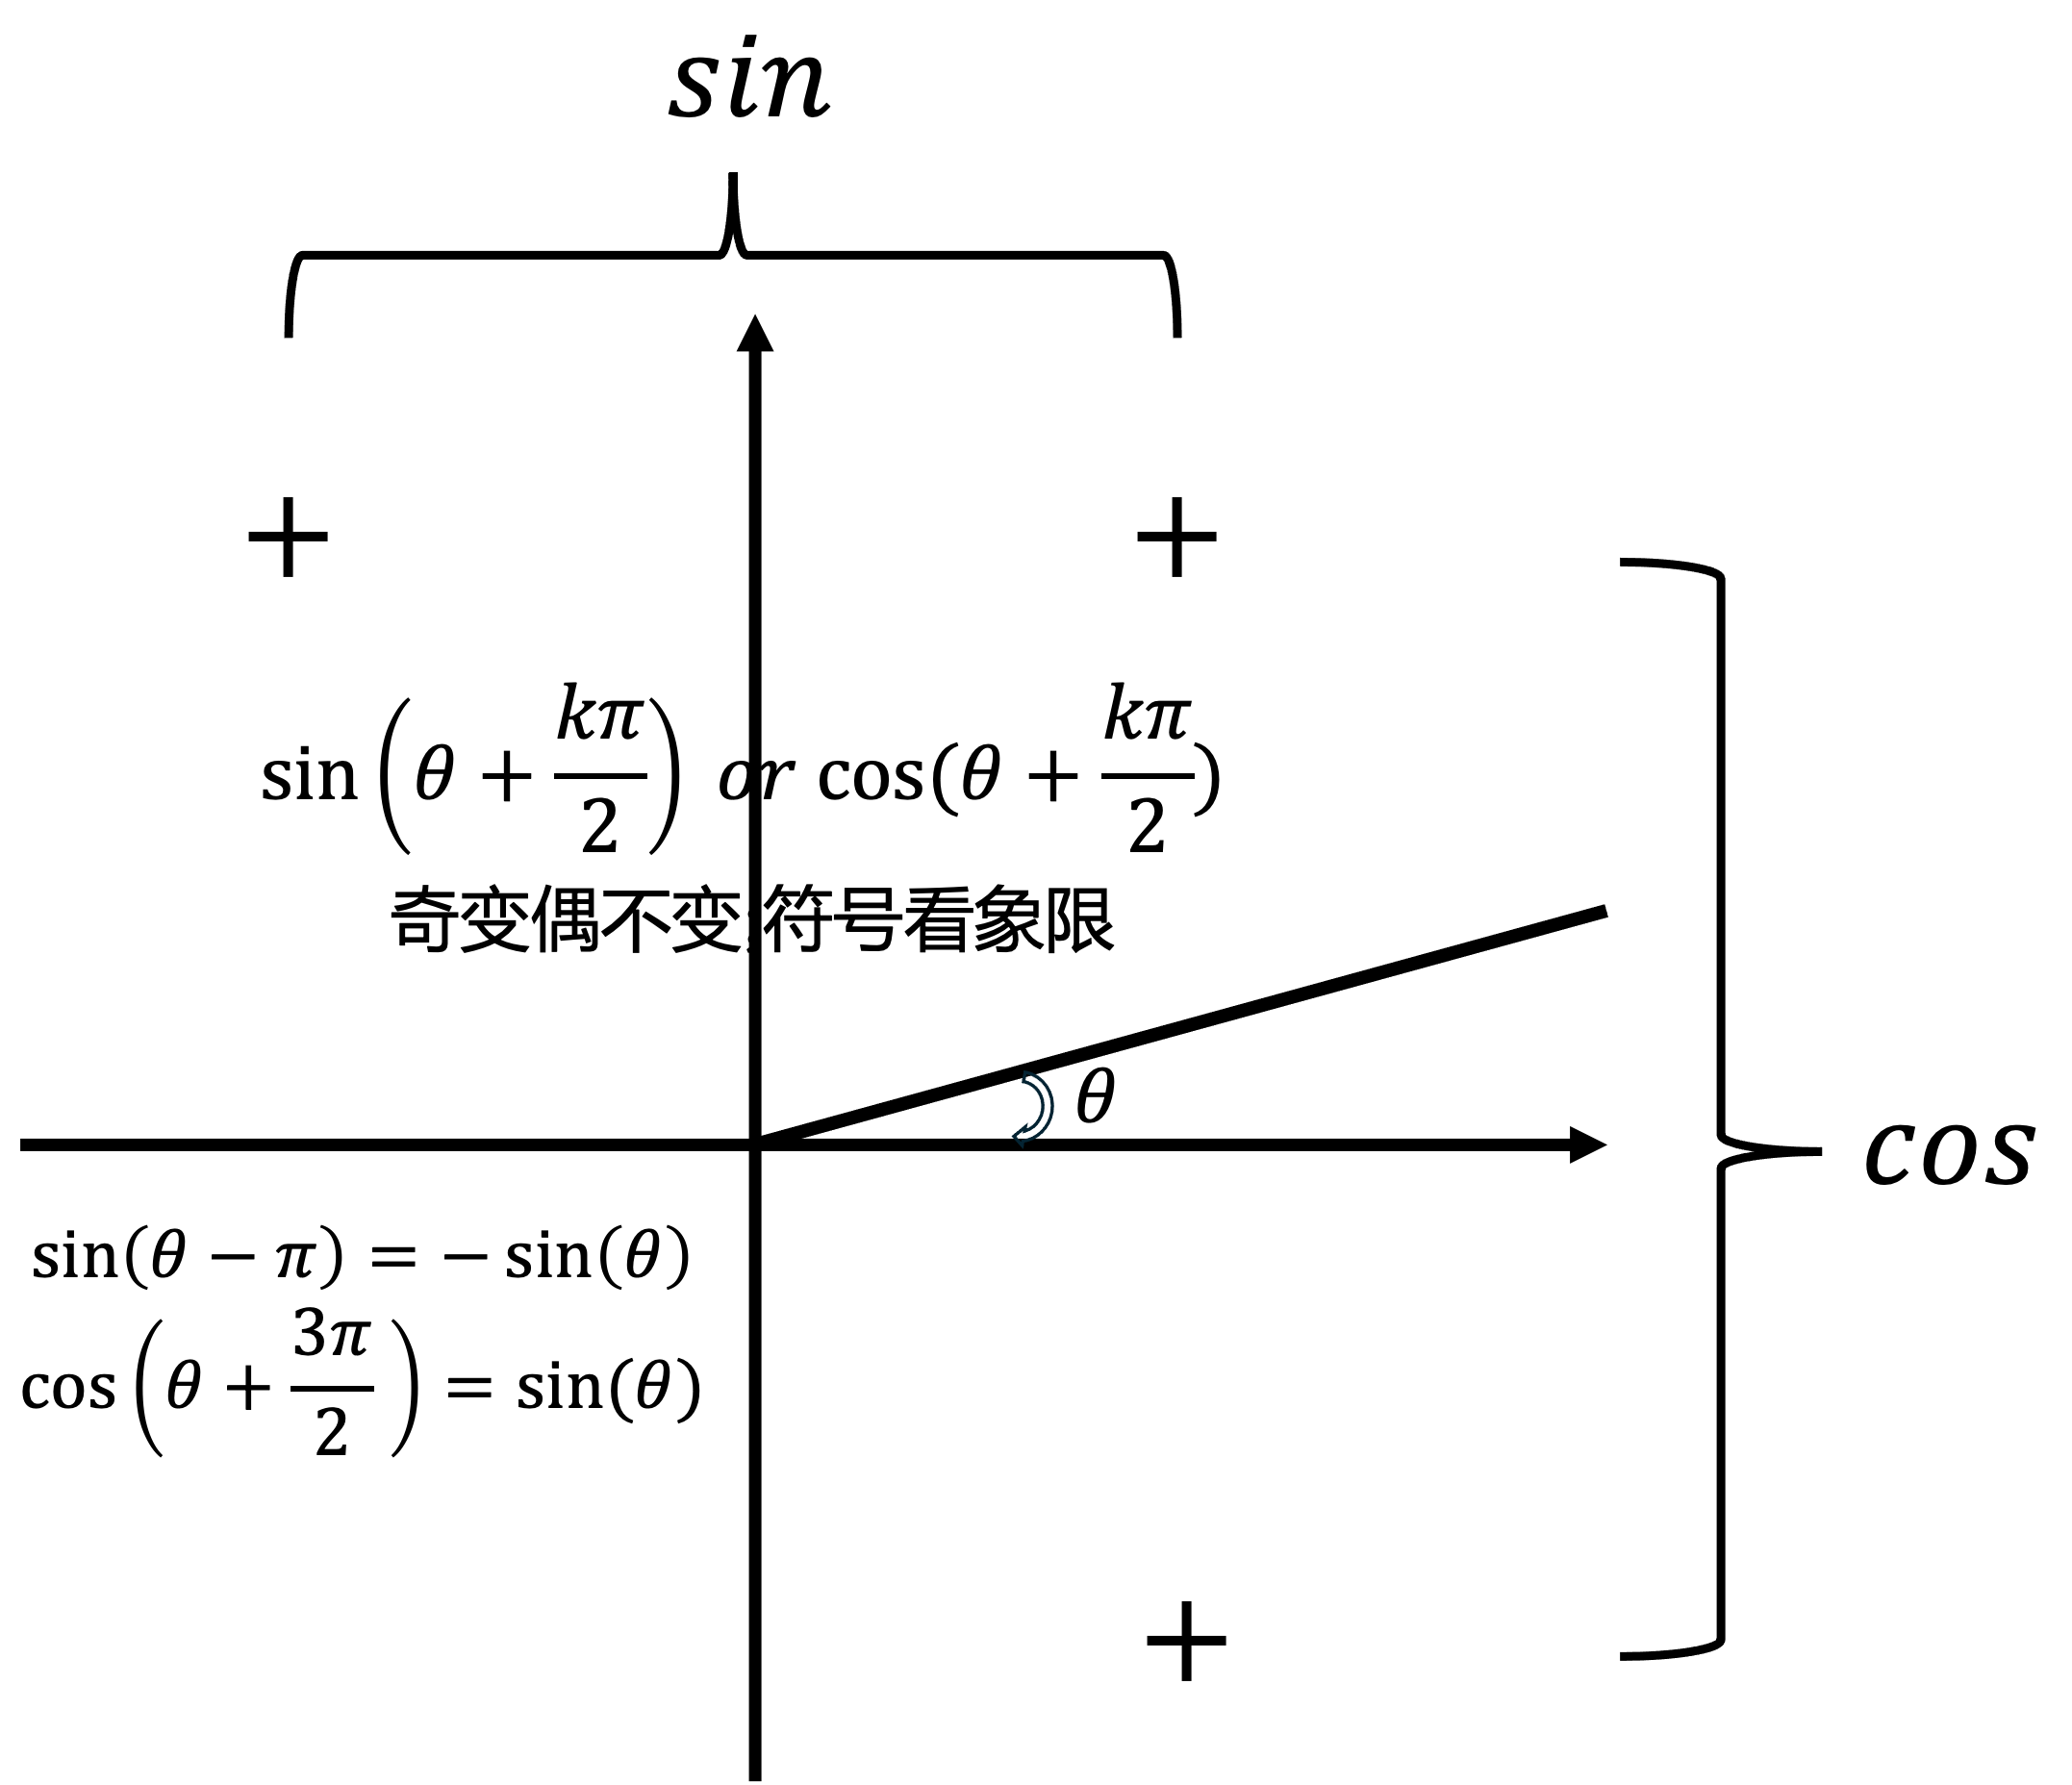
\includegraphics[width = 20em]{./pictures/1.png}

        \item 和关系
              $$ \sin^{2}{\theta}+\cos^{2}{\theta} = 1$$

        \item 正弦定理
              $$ \dfrac{a}{\sin{\alpha}} = \dfrac{b}{\sin{\beta}} = \dfrac{c}{\sin{\gamma}}   $$

        \item 余弦定理
              $$ \cos{\gamma} = \dfrac{a^{2}+b^{2} - c^{2}}{2ab} $$

        \item 二倍角
              $$ \sin{2\theta} = 2\sin{\theta}\cos{\theta} \quad \cos{2\theta} = \cos^{2}{\theta} - \sin^{2}{\theta} \quad \tan{2\theta} = \dfrac{2\tan{\theta}}{1-\tan^{2}{\theta}}$$

        \item 降次
              $$ \sin^{2}{\theta} = \dfrac{1 - \cos{2\theta}}{2} \quad \cos^{2}{\theta} = \dfrac{1 + \cos{2\theta}}{2} \quad \tan^{2}{\theta} = \dfrac{1-\cos{2\theta}}{1+\cos{2\theta}}$$
    \end{itemize}
\end{formal}

\vspace{2em}

\vspace{2em}

\section{光学}
\subsection{折射率}

\begin{itemize}
    \item 定义式:
          $$
              n = \dfrac{\sin{\text{大角}}}{\sin{\text{小角}}}
          $$
    \item 决定式:
          $$
              n = \dfrac{c}{v}
          $$
    \item 全反射:
          \begin{align*}
               & \text{光密介质} \, \ra \, \text{光疏介质} \quad \sin{\text{大角}} = 1 \,(\text{大角} = \frac{\pi}{2}) \\
               & \text{临界角} \quad \sin{C} = \frac{1}{\sin{\text{小角}}}
          \end{align*}
    \item 视深与视高:
          \begin{itemize}
              \item[] $H$为物点距离界面的高度;\,$h$为像点距离界面的高度
              \item 视深: \quad
                    从介质外看向介质内 \quad $h = \frac{1}{n} H$
              \item 视高: \quad
                    从介质内看向介质外 \quad $ h = n H $
          \end{itemize}
    \item 实验误差分析:
          \begin{itemize}
              \item 非平行玻璃砖 $\quad n_{\text{测}} = n_{\text{真}}$
              \item 整体平移  $\quad d_{\text{测}} = d_{\text{玻}} \quad n_{\text{测}} = n_{\text{真}}$
              \item 其他情况  $\quad n_{\text{测}} \text{和} n_{\text{真}} \text{的大小关系} \,\text{与}\, d_{\text{测}} \text{和} d_{\text{玻}}\text{的大小关系相反}$
          \end{itemize}
\end{itemize}

\vspace{2em}

\subsection{干涉实验}
\begin{itemize}
    \item[] 薄膜干涉: $\delta = 2d$
        \begin{itemize}
            \item[] 明暗条纹位置由波长和此处厚度共同决定
            \item[] 相邻明(暗)条纹对应的薄膜厚度差为$\frac{\lambda}{2} \quad \lambda$应为光在介质中传播时的波长
        \end{itemize}
    \item[] 劈尖干涉: 样板下表面和被检查平面的上表面的反射光发生干涉

        \hspace{5em}(标准板的厚度太厚大于相干长度)

        \begin{itemize}
            \item[] 验平问题:
                \begin{itemize}
                    \item[] 若待测板平整,干涉条纹等距
                    \item[] 若条纹\textbf{偏头},则条纹提前出现,此处光程差偏大,因此待测样板此处凹
                    \item[] 若条纹\textbf{偏尾},则条纹延后,此处光程差偏小,因此待测样板此处凸
                \end{itemize}
            \item[] 条纹间距问题:
                \begin{itemize}
                    \item[] 薄片(支撑两个板)的移动改变$\theta$角 $\quad \triangle l = \dfrac{\triangle d}{\tan{\theta}} \quad
                            \triangle d = f(\lambda) = \dfrac{\lambda}{2}$
                \end{itemize}
            \item[] 增反膜;增透膜: 入射光能量 = 折射光能量 + 反射光能量

                \hspace{4em}(注:光疏到光密反射光产生半波损失,$n_{\text{膜}}$介于空气和另一介质之间)

                \hspace{4em}增透膜:反射光相消$2d = \frac{\lambda}{2} (2n+1)$

                \hspace{4em}增反膜:反射光相长$2d = \frac{\lambda}{2} (2n) $
        \end{itemize}

    \item[] 双缝干涉: $\triangle d = \lambda \dfrac{L}{d} \,$ (条纹间距$\triangle d $,双缝间距$d$,缝板距离$L$)
\end{itemize}

\vspace{2em}

\subsection{总结}
\begin{formal}
    符号说明

    \begin{tabular}{|c|c|c|c|c|c|c|c|c|c|}
        \hline
        频率  & 折射率 & 速度  & 临界角 & 波长        & 动量  & 干涉            & 能量            & 逸出功     & 逃逸光子动能  \\
        \hline
        $f$ & $n$ & $v$ & $C$ & $\lambda$ & $p$ & $\triangle x$ & $\varepsilon$ & $w_{0}$ & $E_{k}$ \\
        \hline
    \end{tabular}

    \vspace*{2em}

    \begin{itemize}
        \item 同一介质中不同频率的光

              \vspace*{1em}
              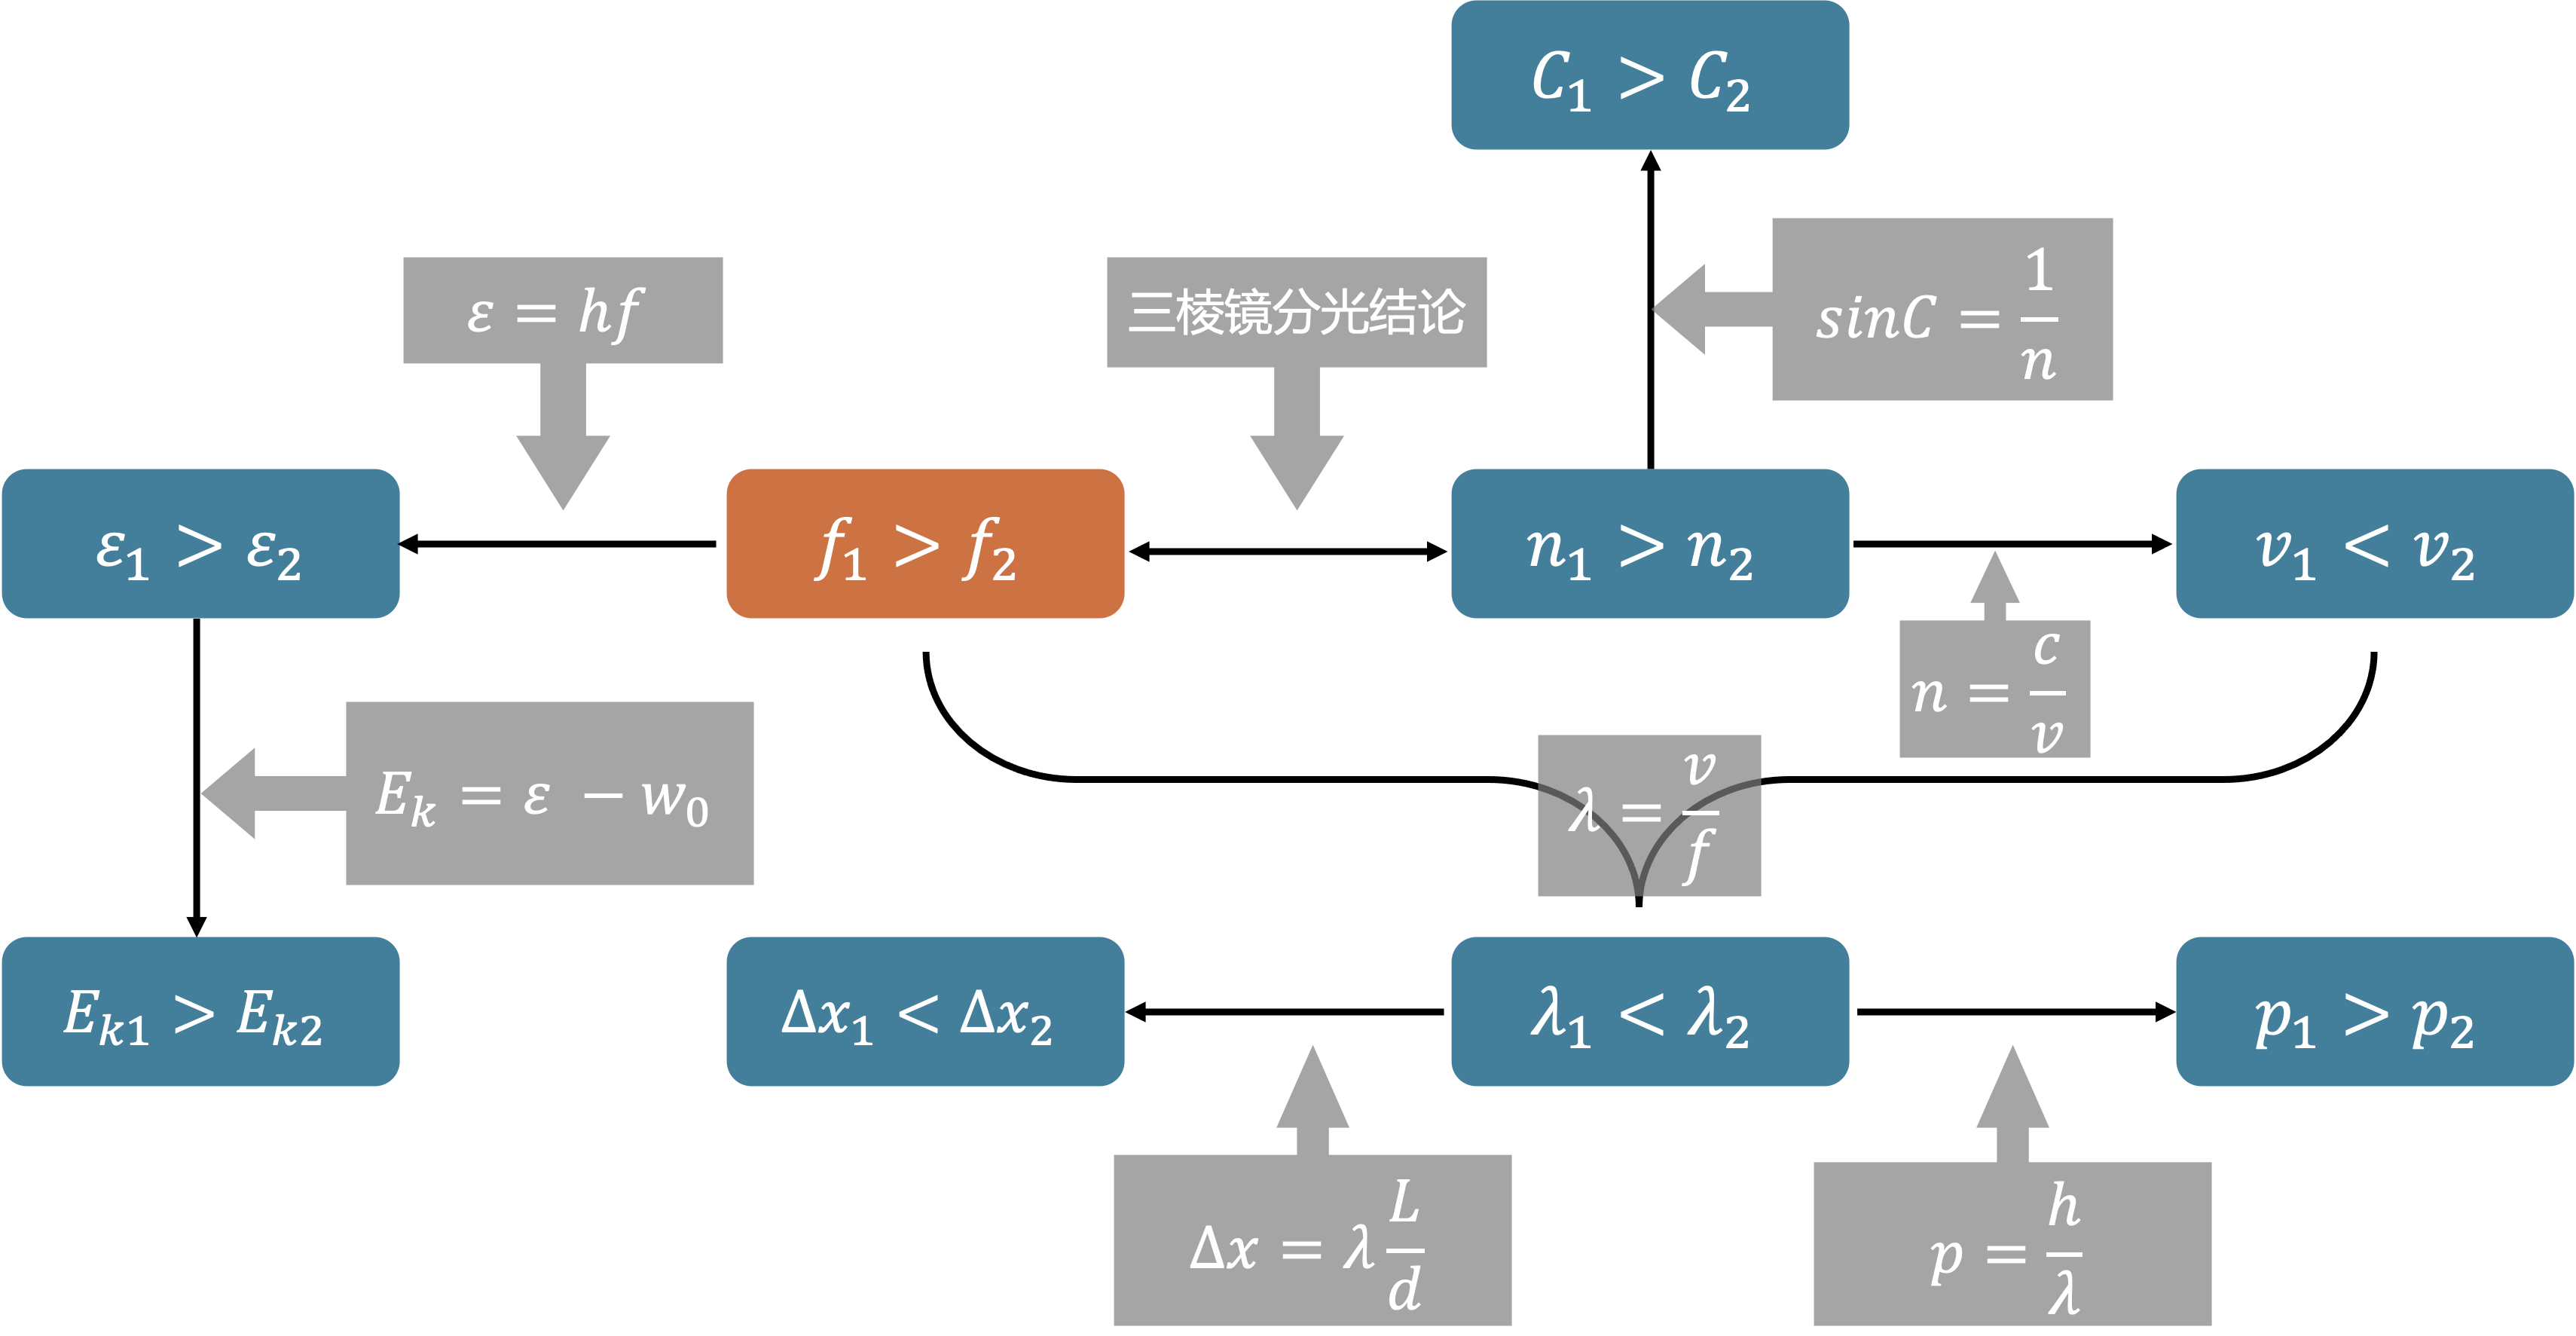
\includegraphics[width=35em,keepaspectratio]{./pictures/2.png}

              \vspace*{2em}

        \item 同一频率的光在不同介质(下标表示不同介质中)中

              \vspace*{1em}
              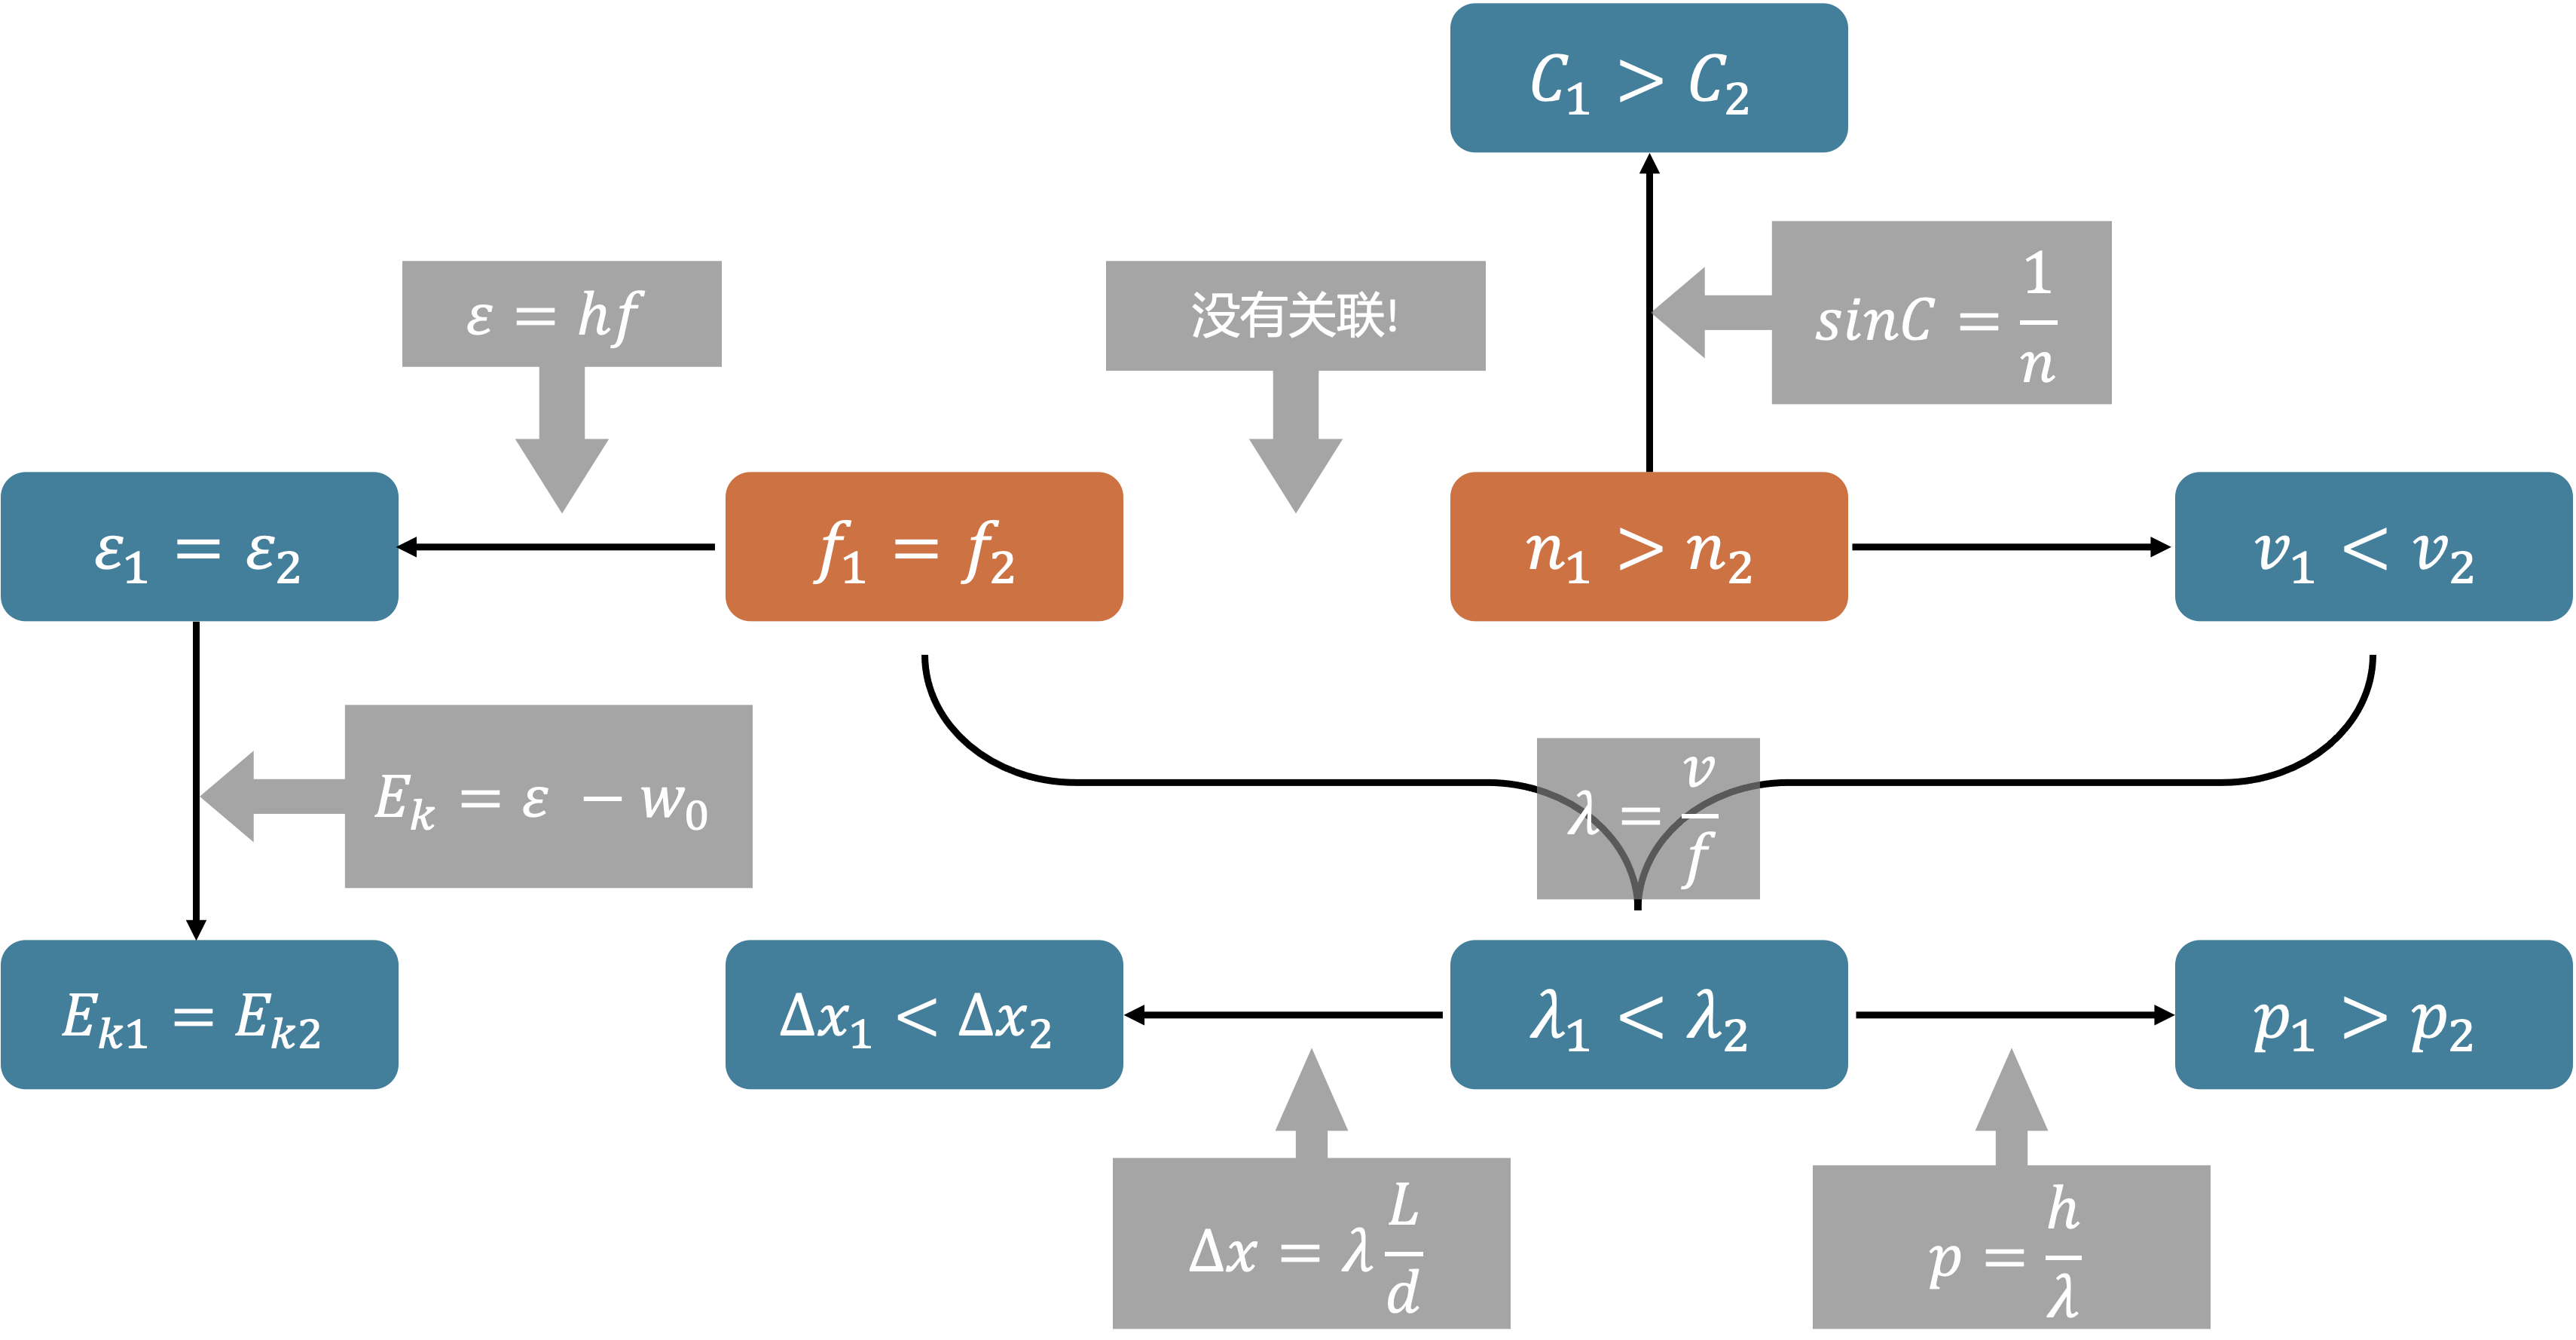
\includegraphics[width=35em,keepaspectratio]{./pictures/3.png}
    \end{itemize}
\end{formal}

\vspace{2em}

\section{热学}
\subsection{黑体辐射}

\subsubsection{物理大厦上的"两朵乌云"}
\begin{itemize}
    \item 迈克尔逊-莫雷实验: 测量假想介质\,\textbf{以太}\,(绝对参考系)$\lra$否定以太得到狭义相对论

          \vspace{1em}

          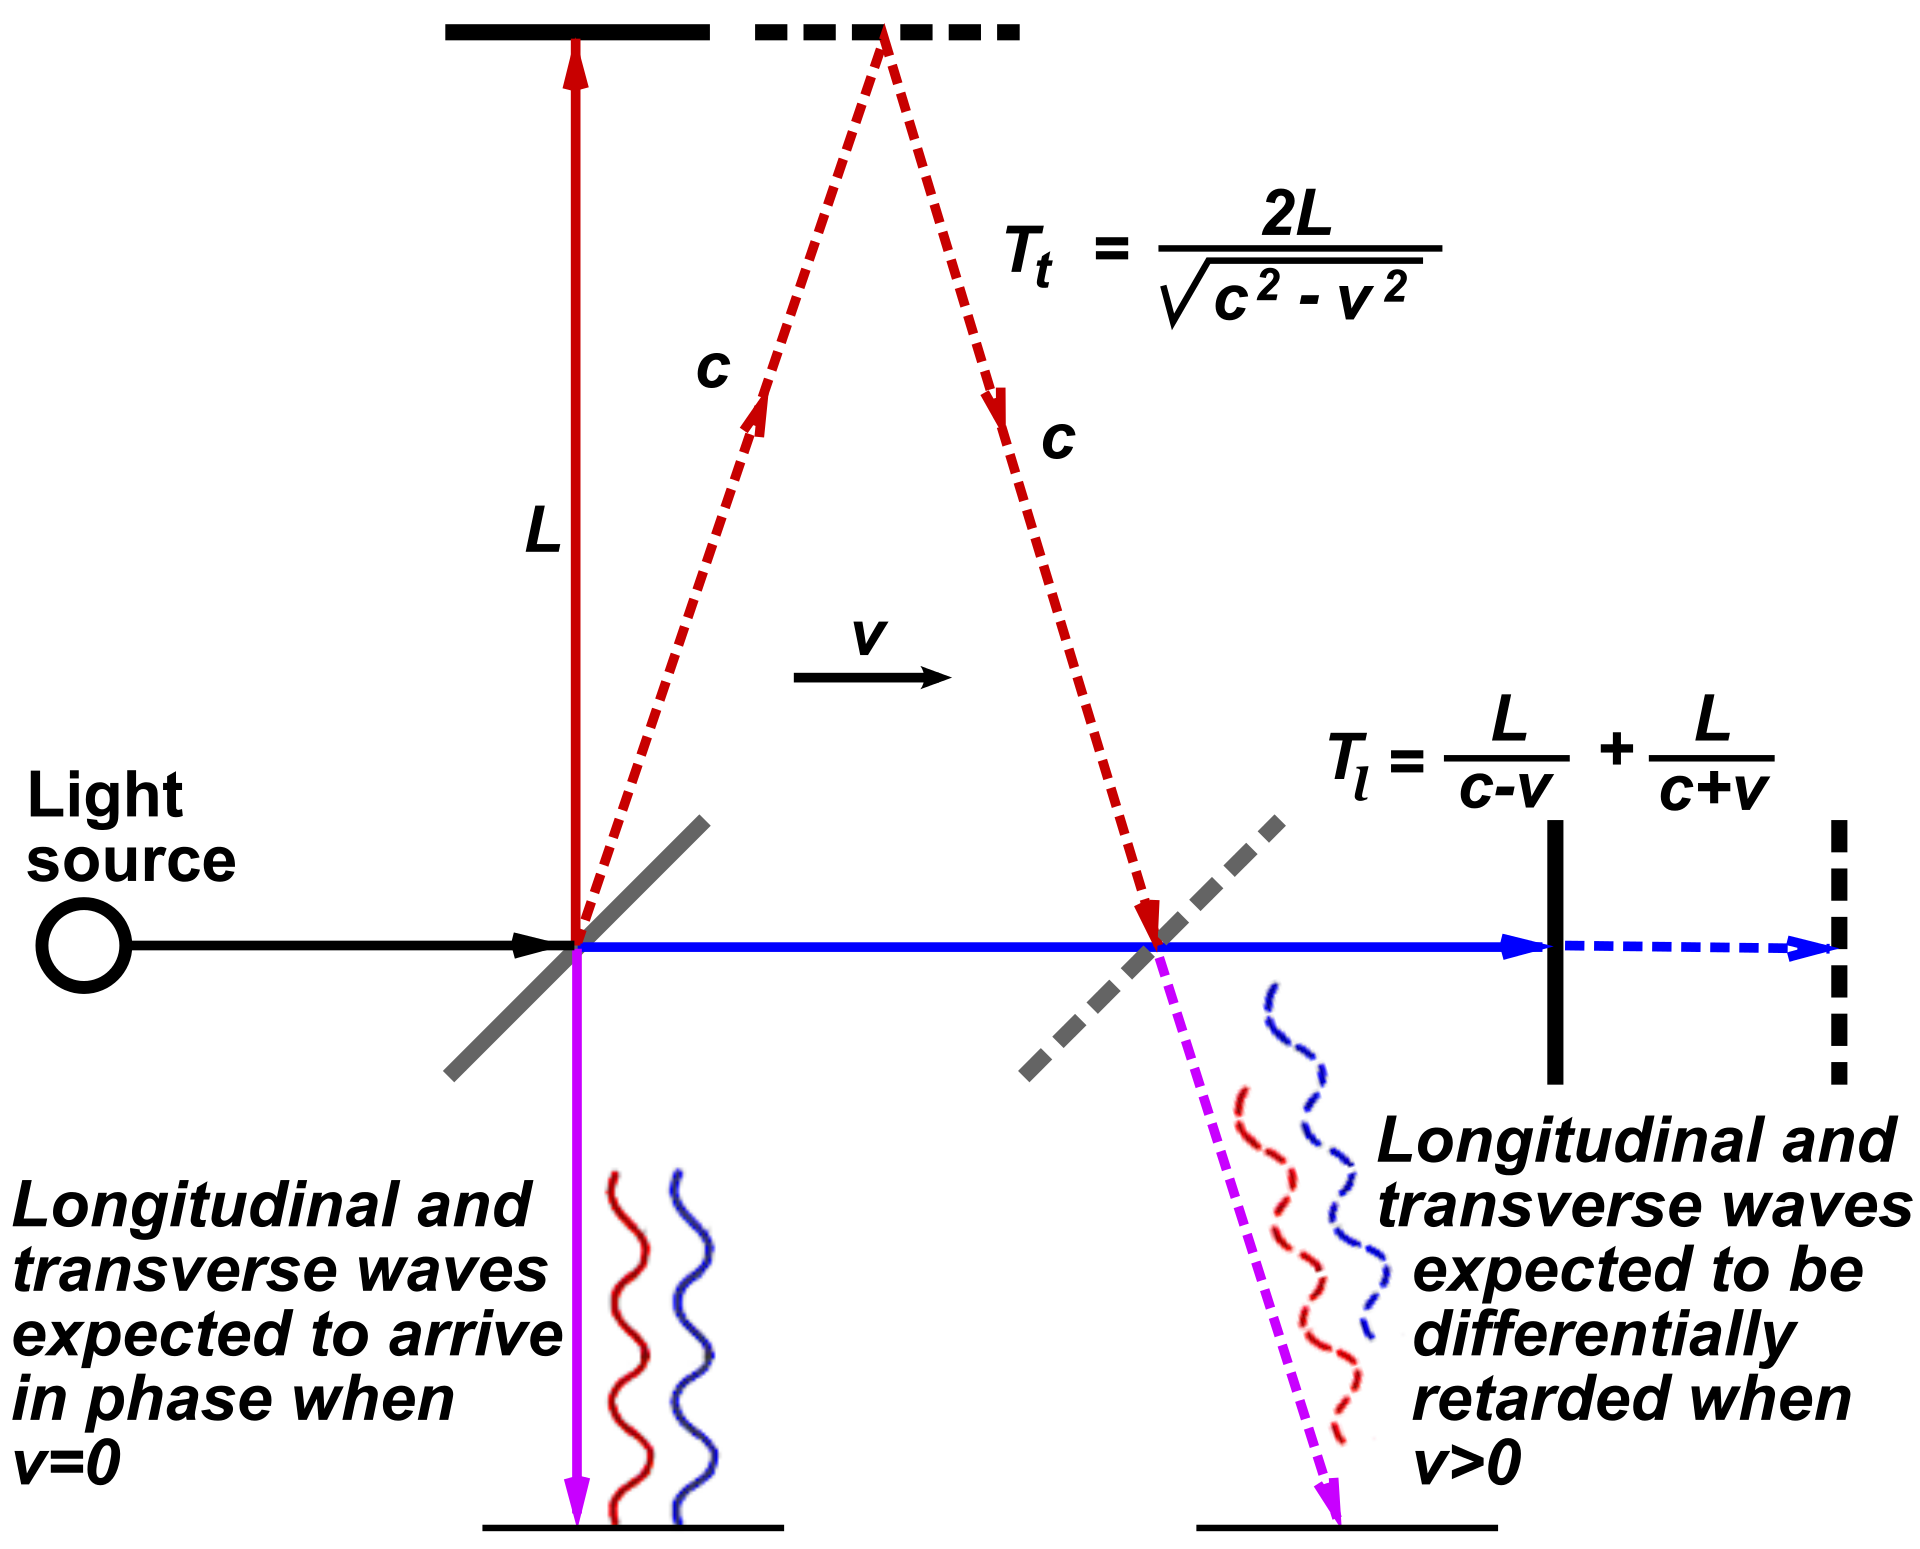
\includegraphics[width=20em,keepaspectratio]{./pictures/4.png}

          \vspace{1em}

    \item 热辐射实验-紫外灾难: 紫外波段辐射能量在当时理论下应为$\infty$,实际辐射能量为$0$
\end{itemize}

\vspace{2em}

\subsubsection{为什么要研究辐射}
\begin{itemize}
    \item 各个国家都在大炼钢铁(大炼钢时代),资本家为了提高炼钢技术请物理学家进行研究
    \item 热辐射: 任何物体都在进行热辐射(电磁波),且与\textbf{温度}(非唯一)有关
    \item 物理学家尝试测量最好炼钢温度所产生的热辐射(电磁波波谱)

          \vspace{2em}

          \begin{minipage}{0.48\textwidth}
              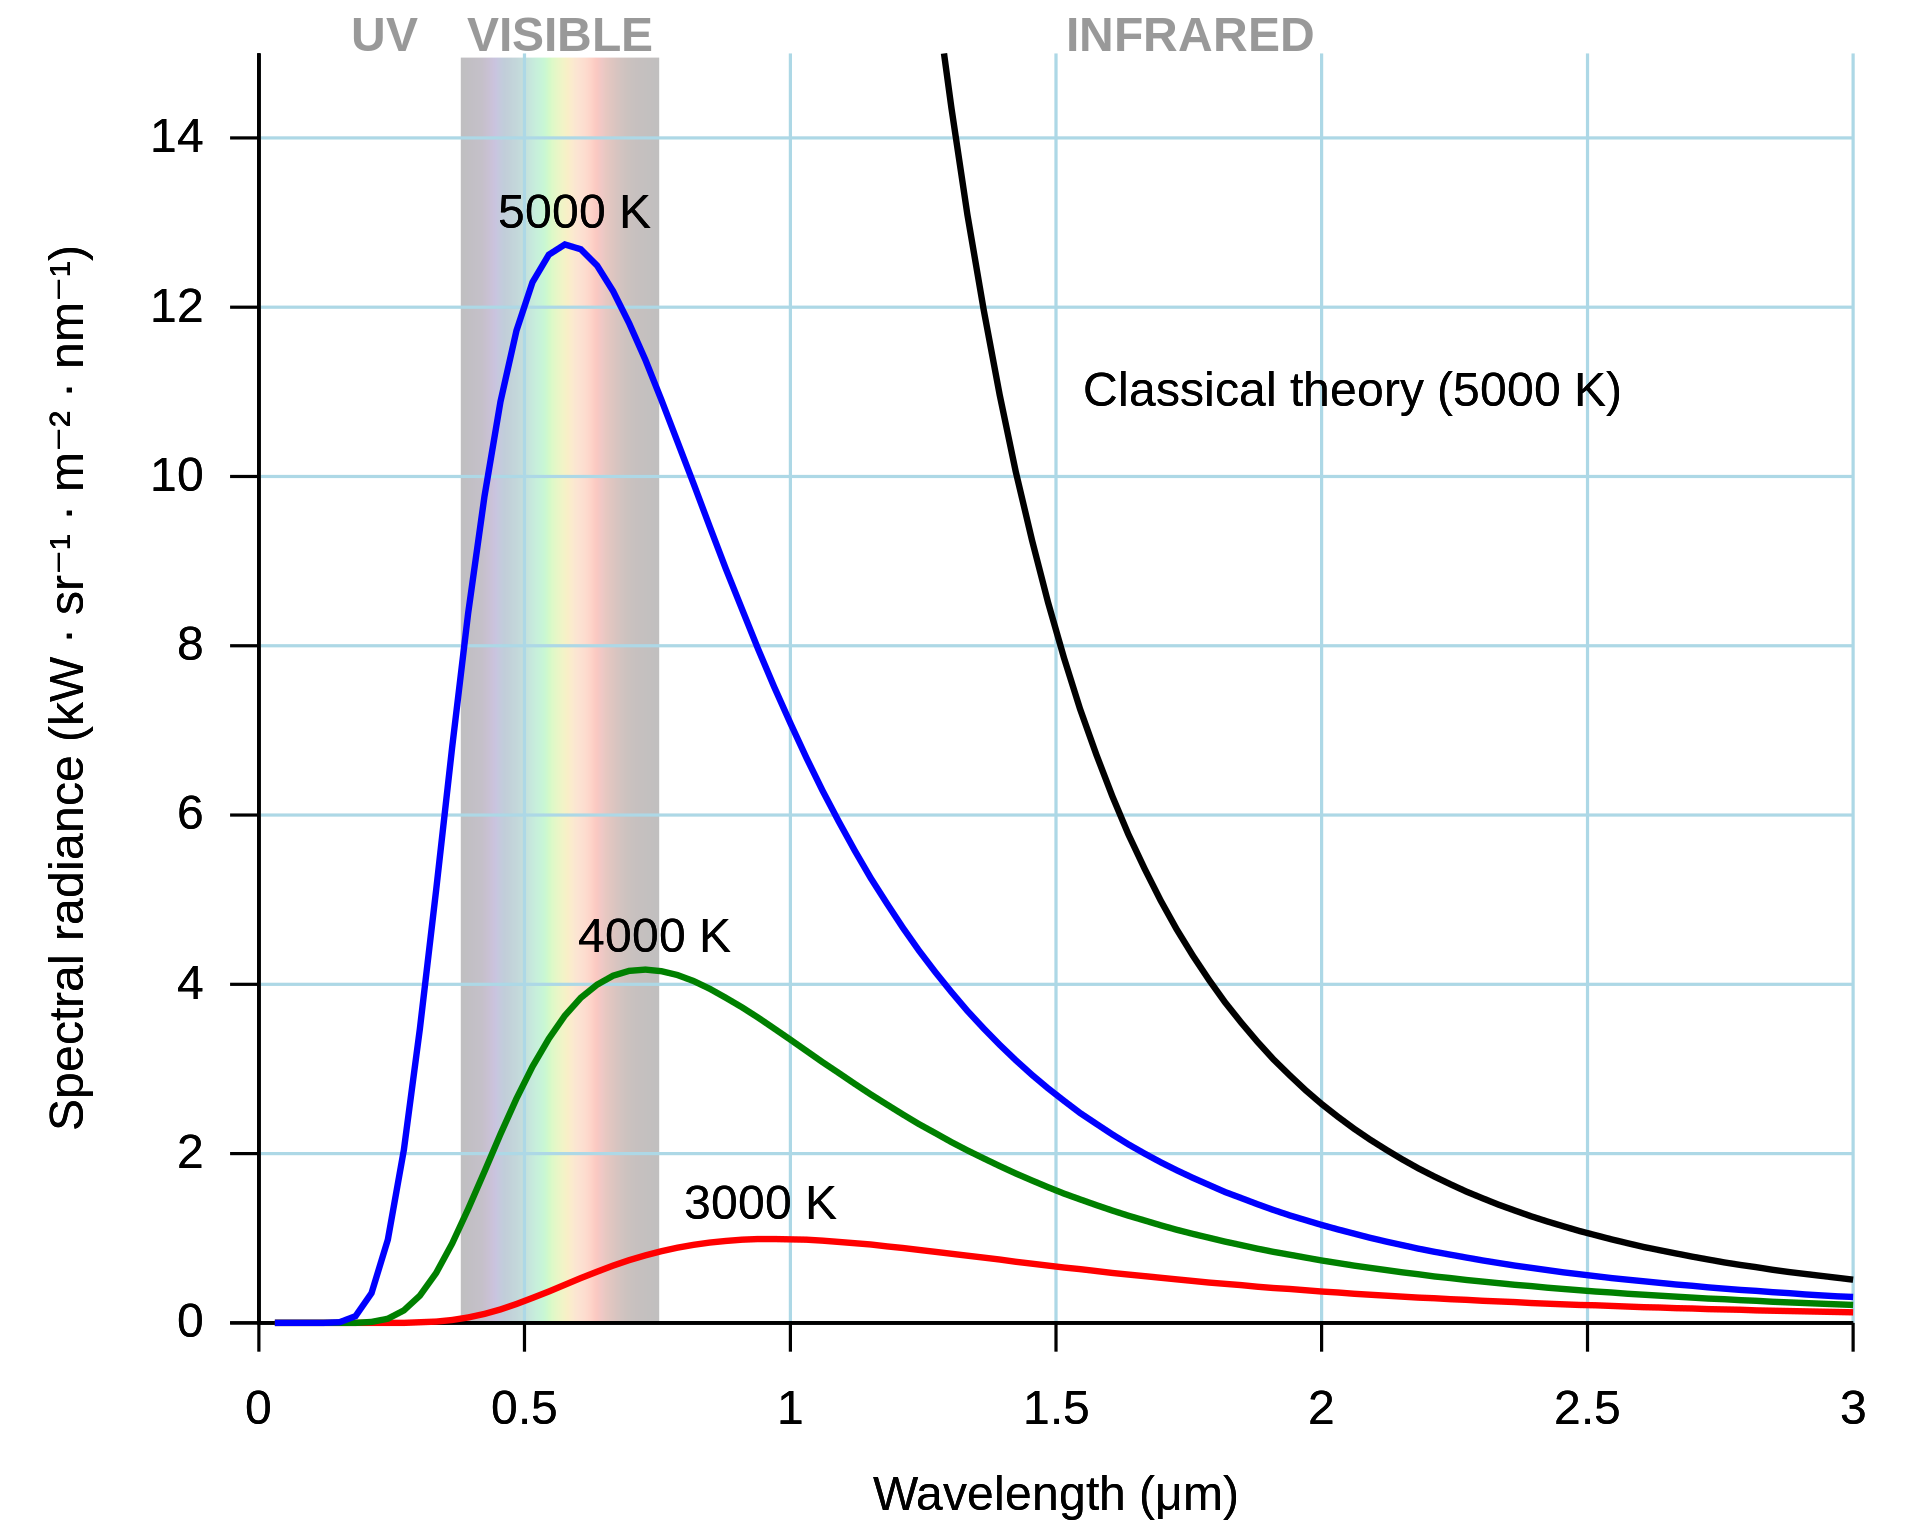
\includegraphics[width=\textwidth,keepaspectratio]{./pictures/5.png}
          \end{minipage}
          \hfill
          \begin{minipage}{0.45\textwidth}
              \vspace{-1em}
              \begin{enumerate}[label = (\arabic*)]
                  \item 在特定温度下,辐射的电磁波波段范围较广,强度不一
                  \item 随着温度的升高,辐射出的各个波段的电磁的辐射强度均升高
                  \item 随着温度升高,辐射强度最强的波长向\textbf{左}移动(频率上升)
              \end{enumerate}
              \vspace{1em}
              \begin{enumerate}[label = (\alph*)]
                  \item 维恩公式(短波接近)
                  \item 瑞利公式(长波接近) $\lra$ 紫外灾难(短波接近无穷)
              \end{enumerate}
          \end{minipage}
\end{itemize}

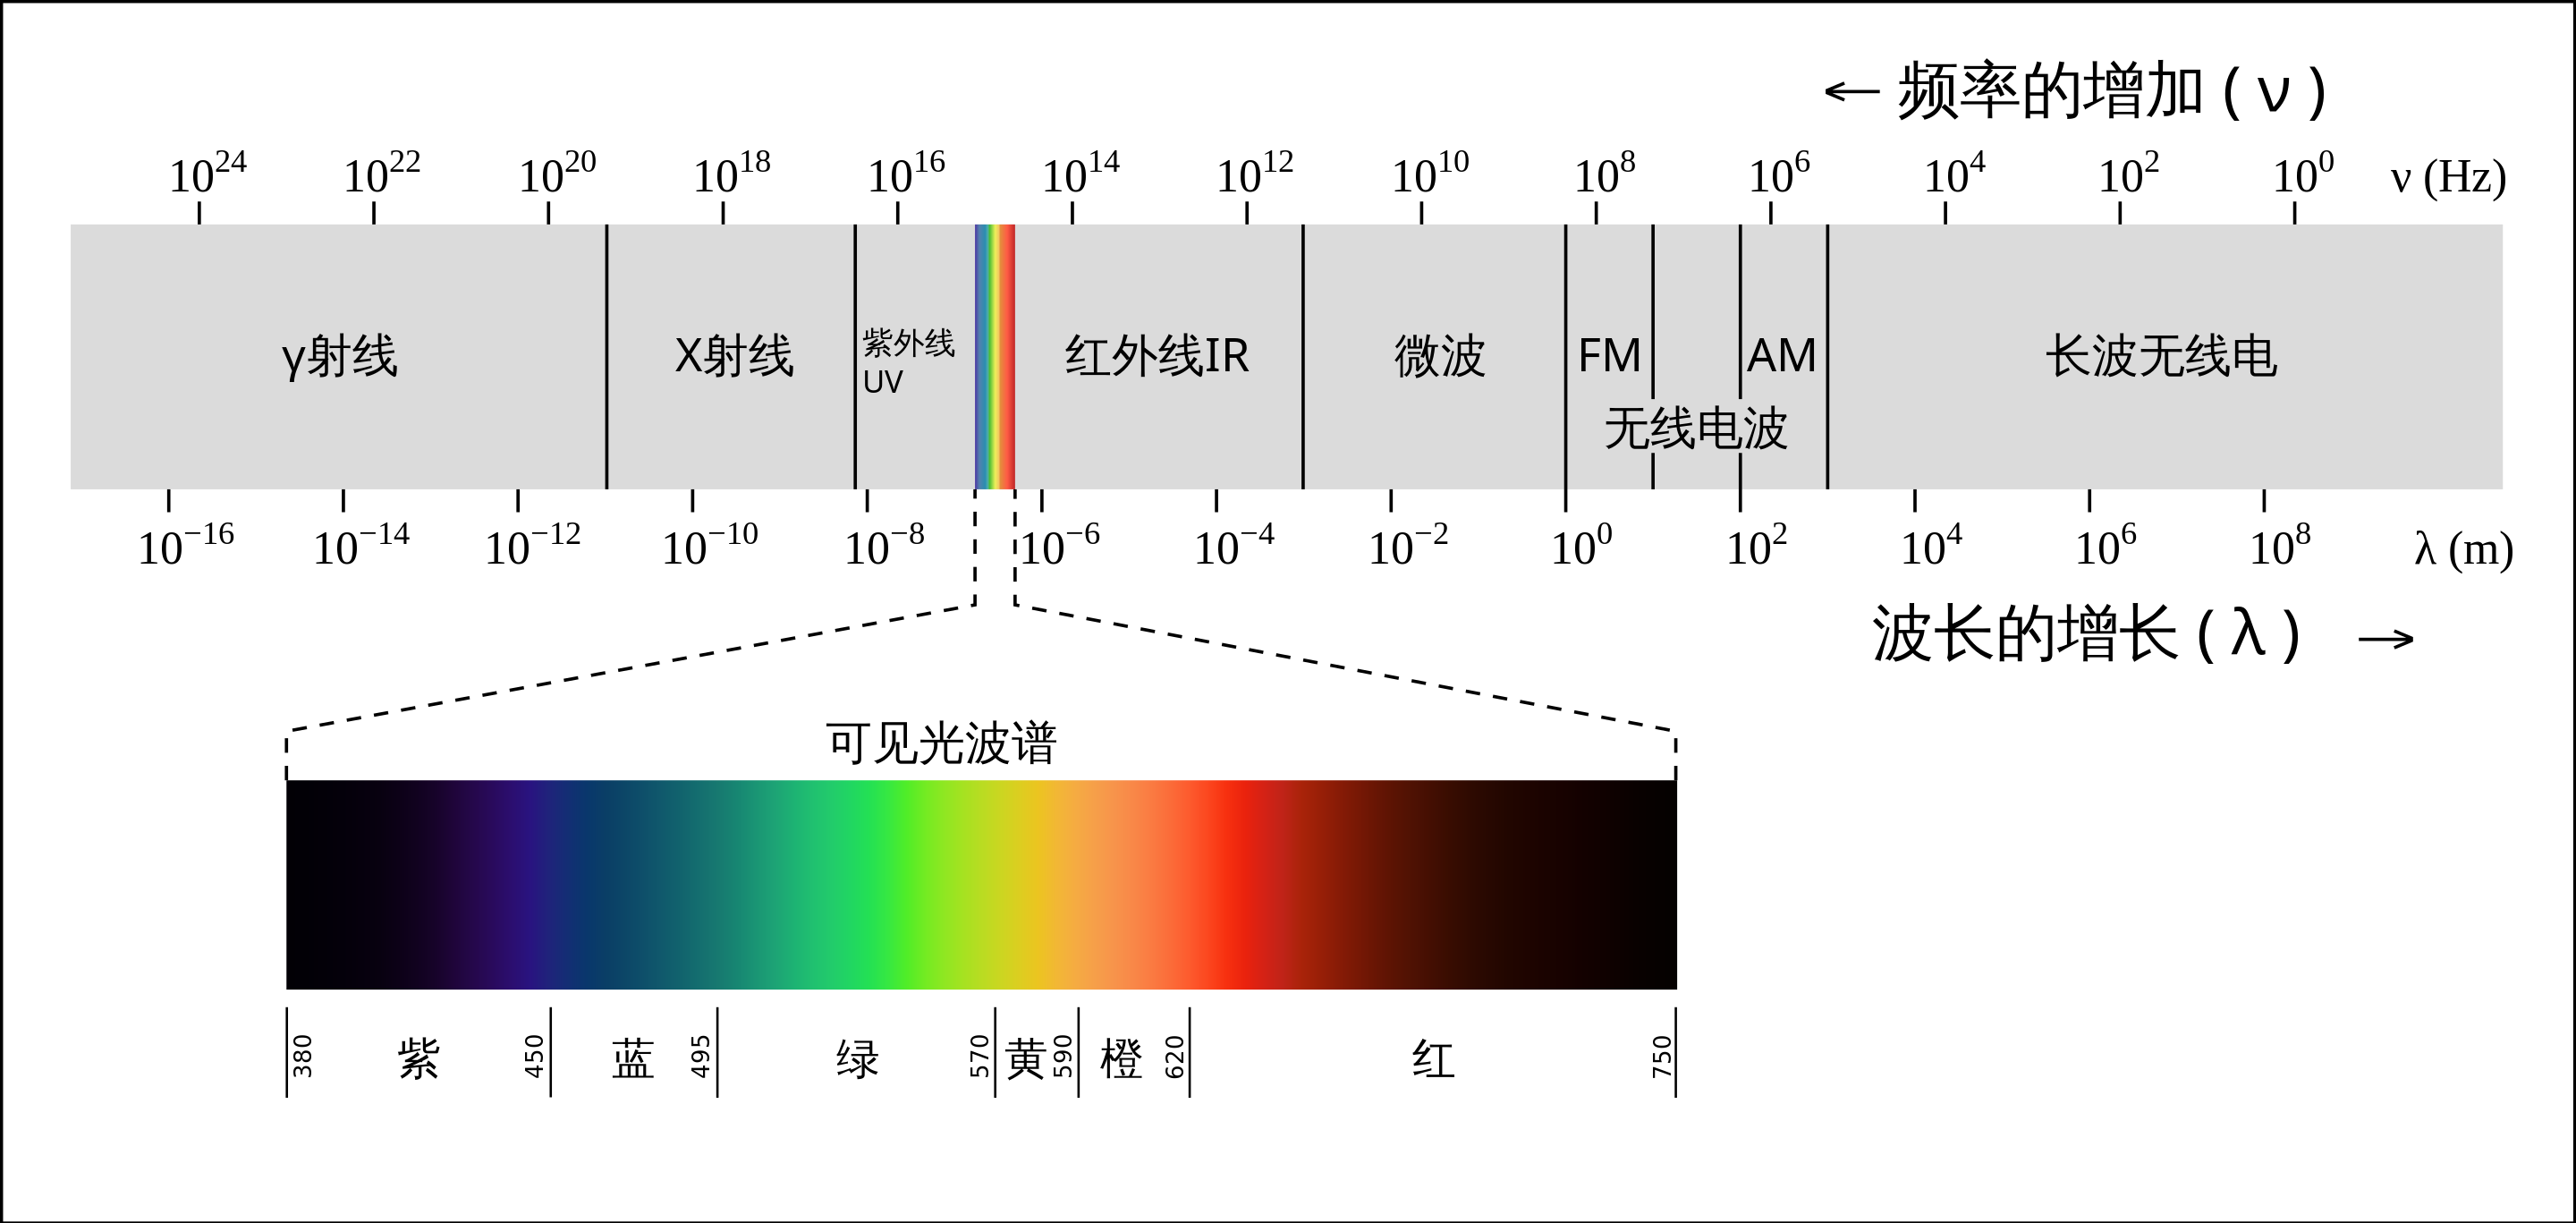
\includegraphics[width=37em,keepaspectratio]{./pictures/6.png}

\vspace{2em}

\subsubsection{黑体模型}
\begin{itemize}
    \item 理想黑体概念: 反射率与透射率为$0$,吸收率$100\%$,全靠自身发射辐射
    \item[] 常见近似黑体: 太阳 \, 发光灯泡 \, 钻孔箱
\end{itemize}

\vspace{2em}

\subsubsection{能量子-普朗克}

\begin{minipage}{0.4\textwidth}
    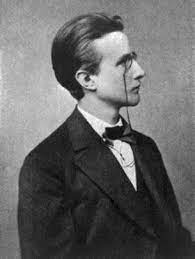
\includegraphics[width=15em,keepaspectratio]{./pictures/7.png}
\end{minipage}
\hfill
\begin{minipage}{0.4\textwidth}
    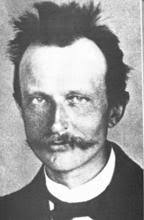
\includegraphics[width=13em,keepaspectratio]{./pictures/8.png}
\end{minipage}

\vspace{2em}

\begin{itemize}
    \item 能量子: 认为带电微粒的能量只能是某一最小能量值的整数倍,最小能量值称之为---能量子
    \item 光子: 爱因斯坦在\textbf{光电效应}现象中认为光本身由一个个不可分割的能量子组成,
          频率为$\nu$的光其能量为$h\nu$,后被称为光子
          $$
              E = h\nu    \hspace{2em}   \text{普朗克常数} \hspace{0.5em} h = 6.63 \cross 10^{-34}
          $$
\end{itemize}

\vspace{2em}

\subsubsection{光的一些描述}
\begin{itemize}
    \item 光速(传播): 真空中传播速度$3 \cross 10^{8}m/s $
    \item 频率(颜色): 单位时间内完成的周期次数$\nu$
    \item 强度(亮度): 单位时间内的光子数(粗浅定义) \, $I = nh\nu$ \, (单一光的强度改变仅改变$n$)
\end{itemize}

\vspace{2em}

\subsection{光电效应}
\subsubsection{理想模型}

\begin{minipage}{0.5\textwidth}
    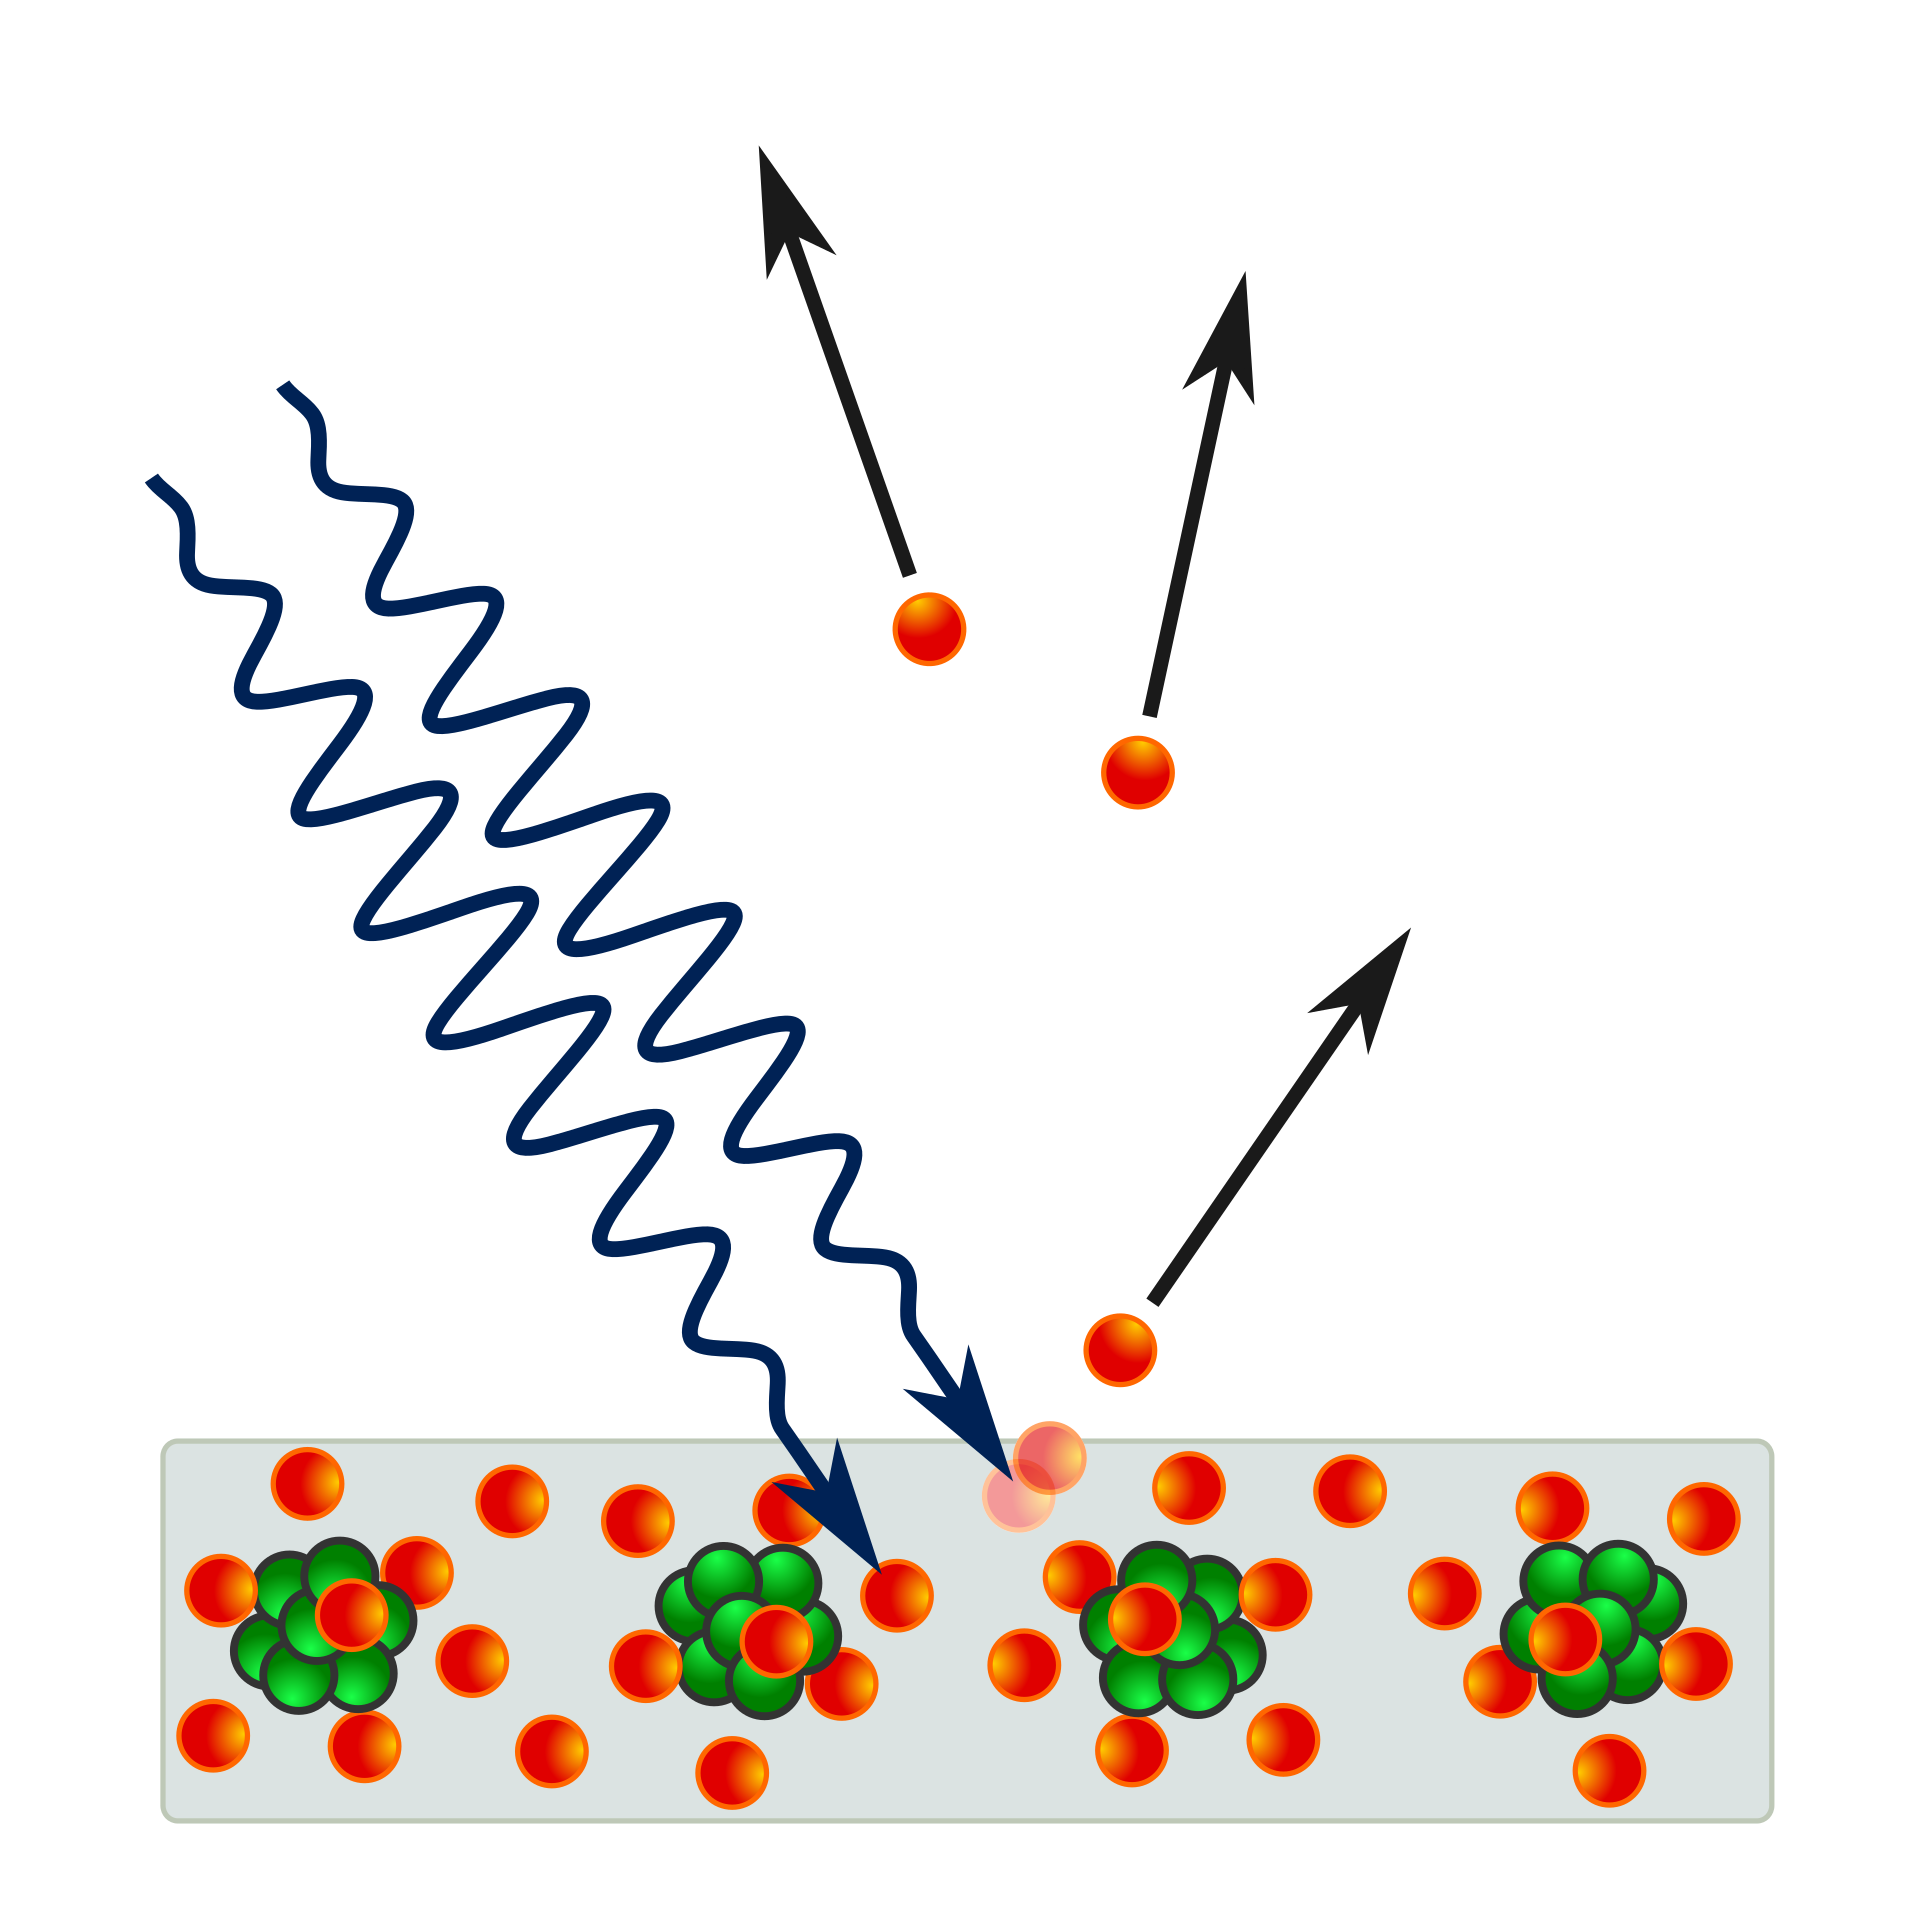
\includegraphics[width=15em,keepaspectratio]{./pictures/9.png}
\end{minipage}
\hspace{-5em}
\begin{minipage}{0.5\textwidth}
    \begin{itemize}
        \item 核外电子处于某能级上,吸收特定能量将会\textbf{跃迁}或\textbf{逃离}(电离)
        \item[]
        \item 单个光子的能量被吸收后仍有\textbf{余量},则作为电子的初动能
        \item[]
        \item 电子逃离在化学中$\llra$被氧化,这也是有些材料需要避光存储的原因
    \end{itemize}
\end{minipage}

\vspace{2em}

\subsubsection{实验雏形}
\begin{minipage}{0.5\textwidth}
    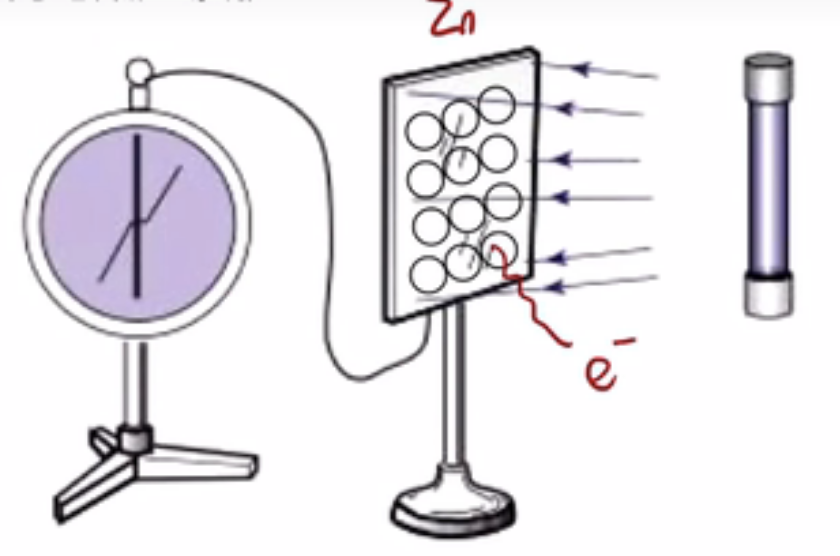
\includegraphics[width=15em,keepaspectratio]{./pictures/10.png}
\end{minipage}
\hspace{-5em}
\begin{minipage}{0.5\textwidth}
    \begin{itemize}
        \item 电子吸收能量逃离
        \item[]
        \item $Zn$板处于\textbf{正电}
        \item[]
        \item 验电器处于\textbf{正电}(工作原理:接触式起电)
    \end{itemize}
\end{minipage}

\vspace{2em}

\subsubsection{电学实验}
\begin{minipage}{0.45 \textwidth}
    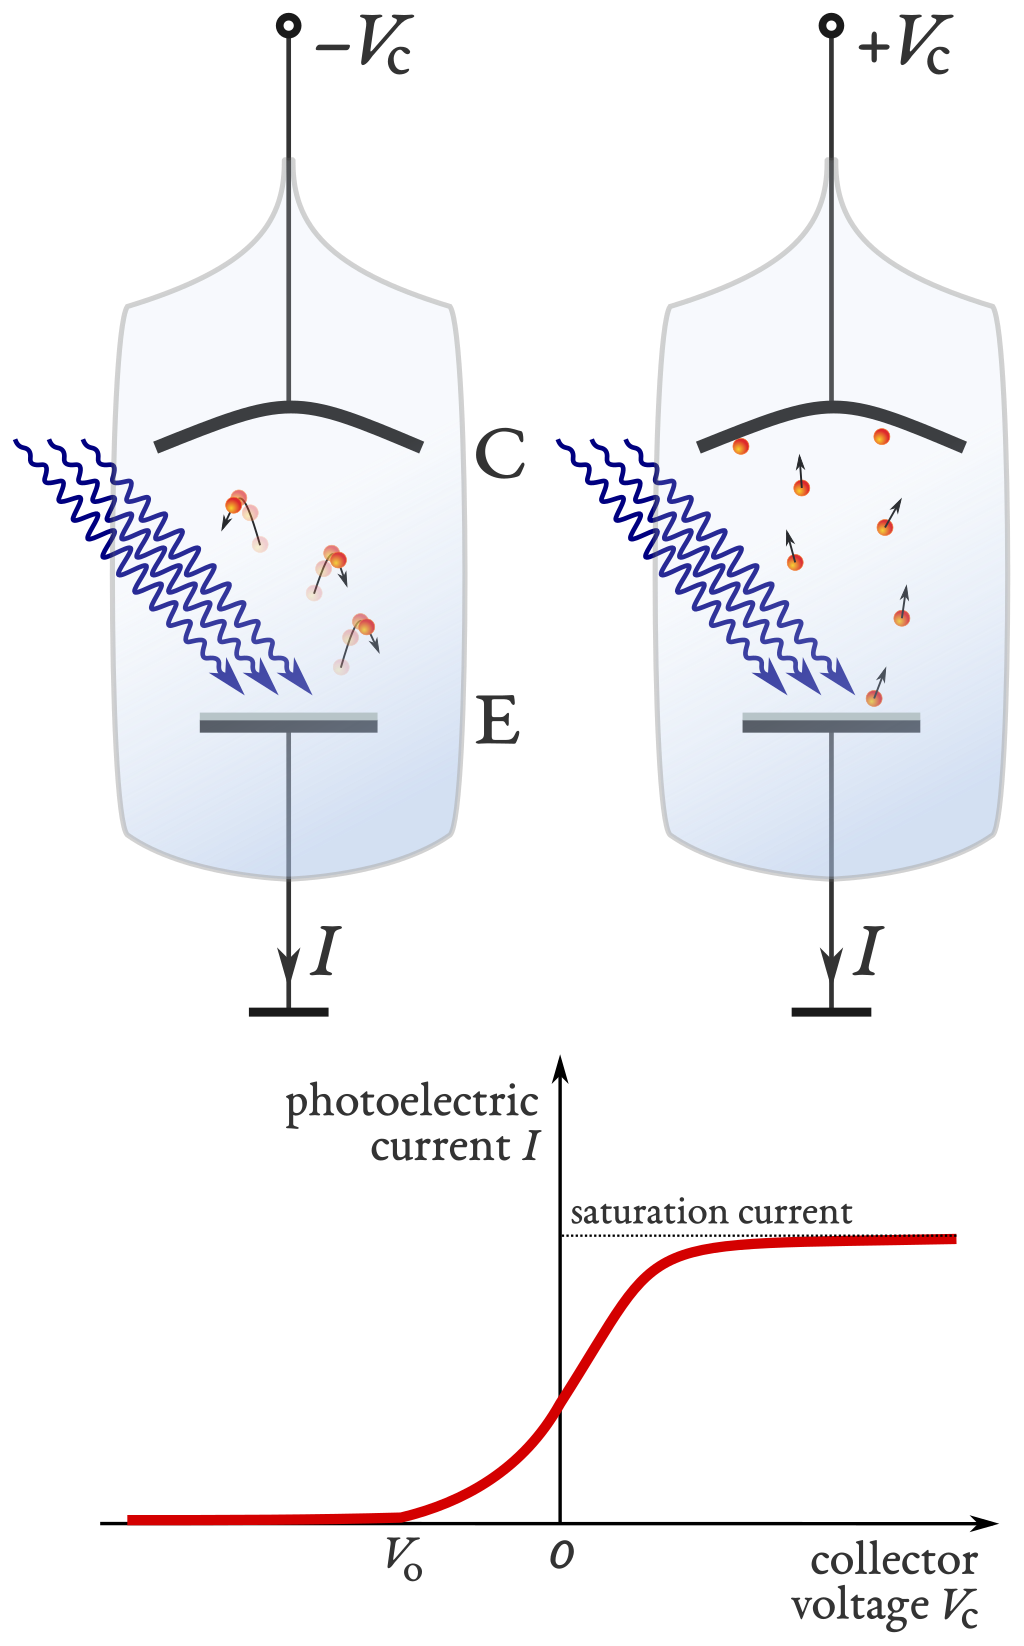
\includegraphics[width=16em,keepaspectratio]{./pictures/11.png}
\end{minipage}
\hspace{-2em}
\begin{minipage}{0.5\textwidth}
    \begin{itemize}
        \item 逸出功: 电子逃逸出金属表面所需要的最小能量 \, $W_{0}$
        \item[]
        \item 最大初动能: 一定频率光照下刚逃逸的电子所具有最大初动能 $E_{kmax} = h\nu - W_{0}$
        \item[]
        \item 饱和光电流: 所有逃逸电子均打到极板(忽略速度对电流的影响) \, $I_{s}$
              \begin{itemize}
                  \item[] 增大光频率 $\times$
                  \item[] 增加光照强度(调整$n$)$\surd$
              \end{itemize}
        \item[]
        \item 遏止电压: 恰好使得没有任何电子打到极板$V_{stop}q = E_{kmax}$ (抵消电子最大初动能)
        \item[]
        \item 截止频率(极限频率): 恰好发生光电效应时的频率$E_{kmax} \lra \nu_{0} = \frac{W_{0}}{h} $
    \end{itemize}
\end{minipage}

\vspace{2em}

\subsection{原子结构}
\subsubsection{物理学史}
\begin{enumerate}
    \item J.J汤姆孙发现了电子: 阴极射线的粒子称为电子
    \item J.J汤姆孙提出\textbf{"枣糕模型"}: 认为原子是一个球体,其中\textbf{正电荷分布均匀,电子镶嵌}其中
    \item 卢瑟福通过\, $\alpha$粒子散射实验 \, 提出\textbf{"核式结构模型"}:所有带正电部分体积很小但几乎有全部质量,电子在外运动

          \begin{figure}[h]
              \centering
              \begin{minipage}{0.48\textwidth}
                  \centering
                  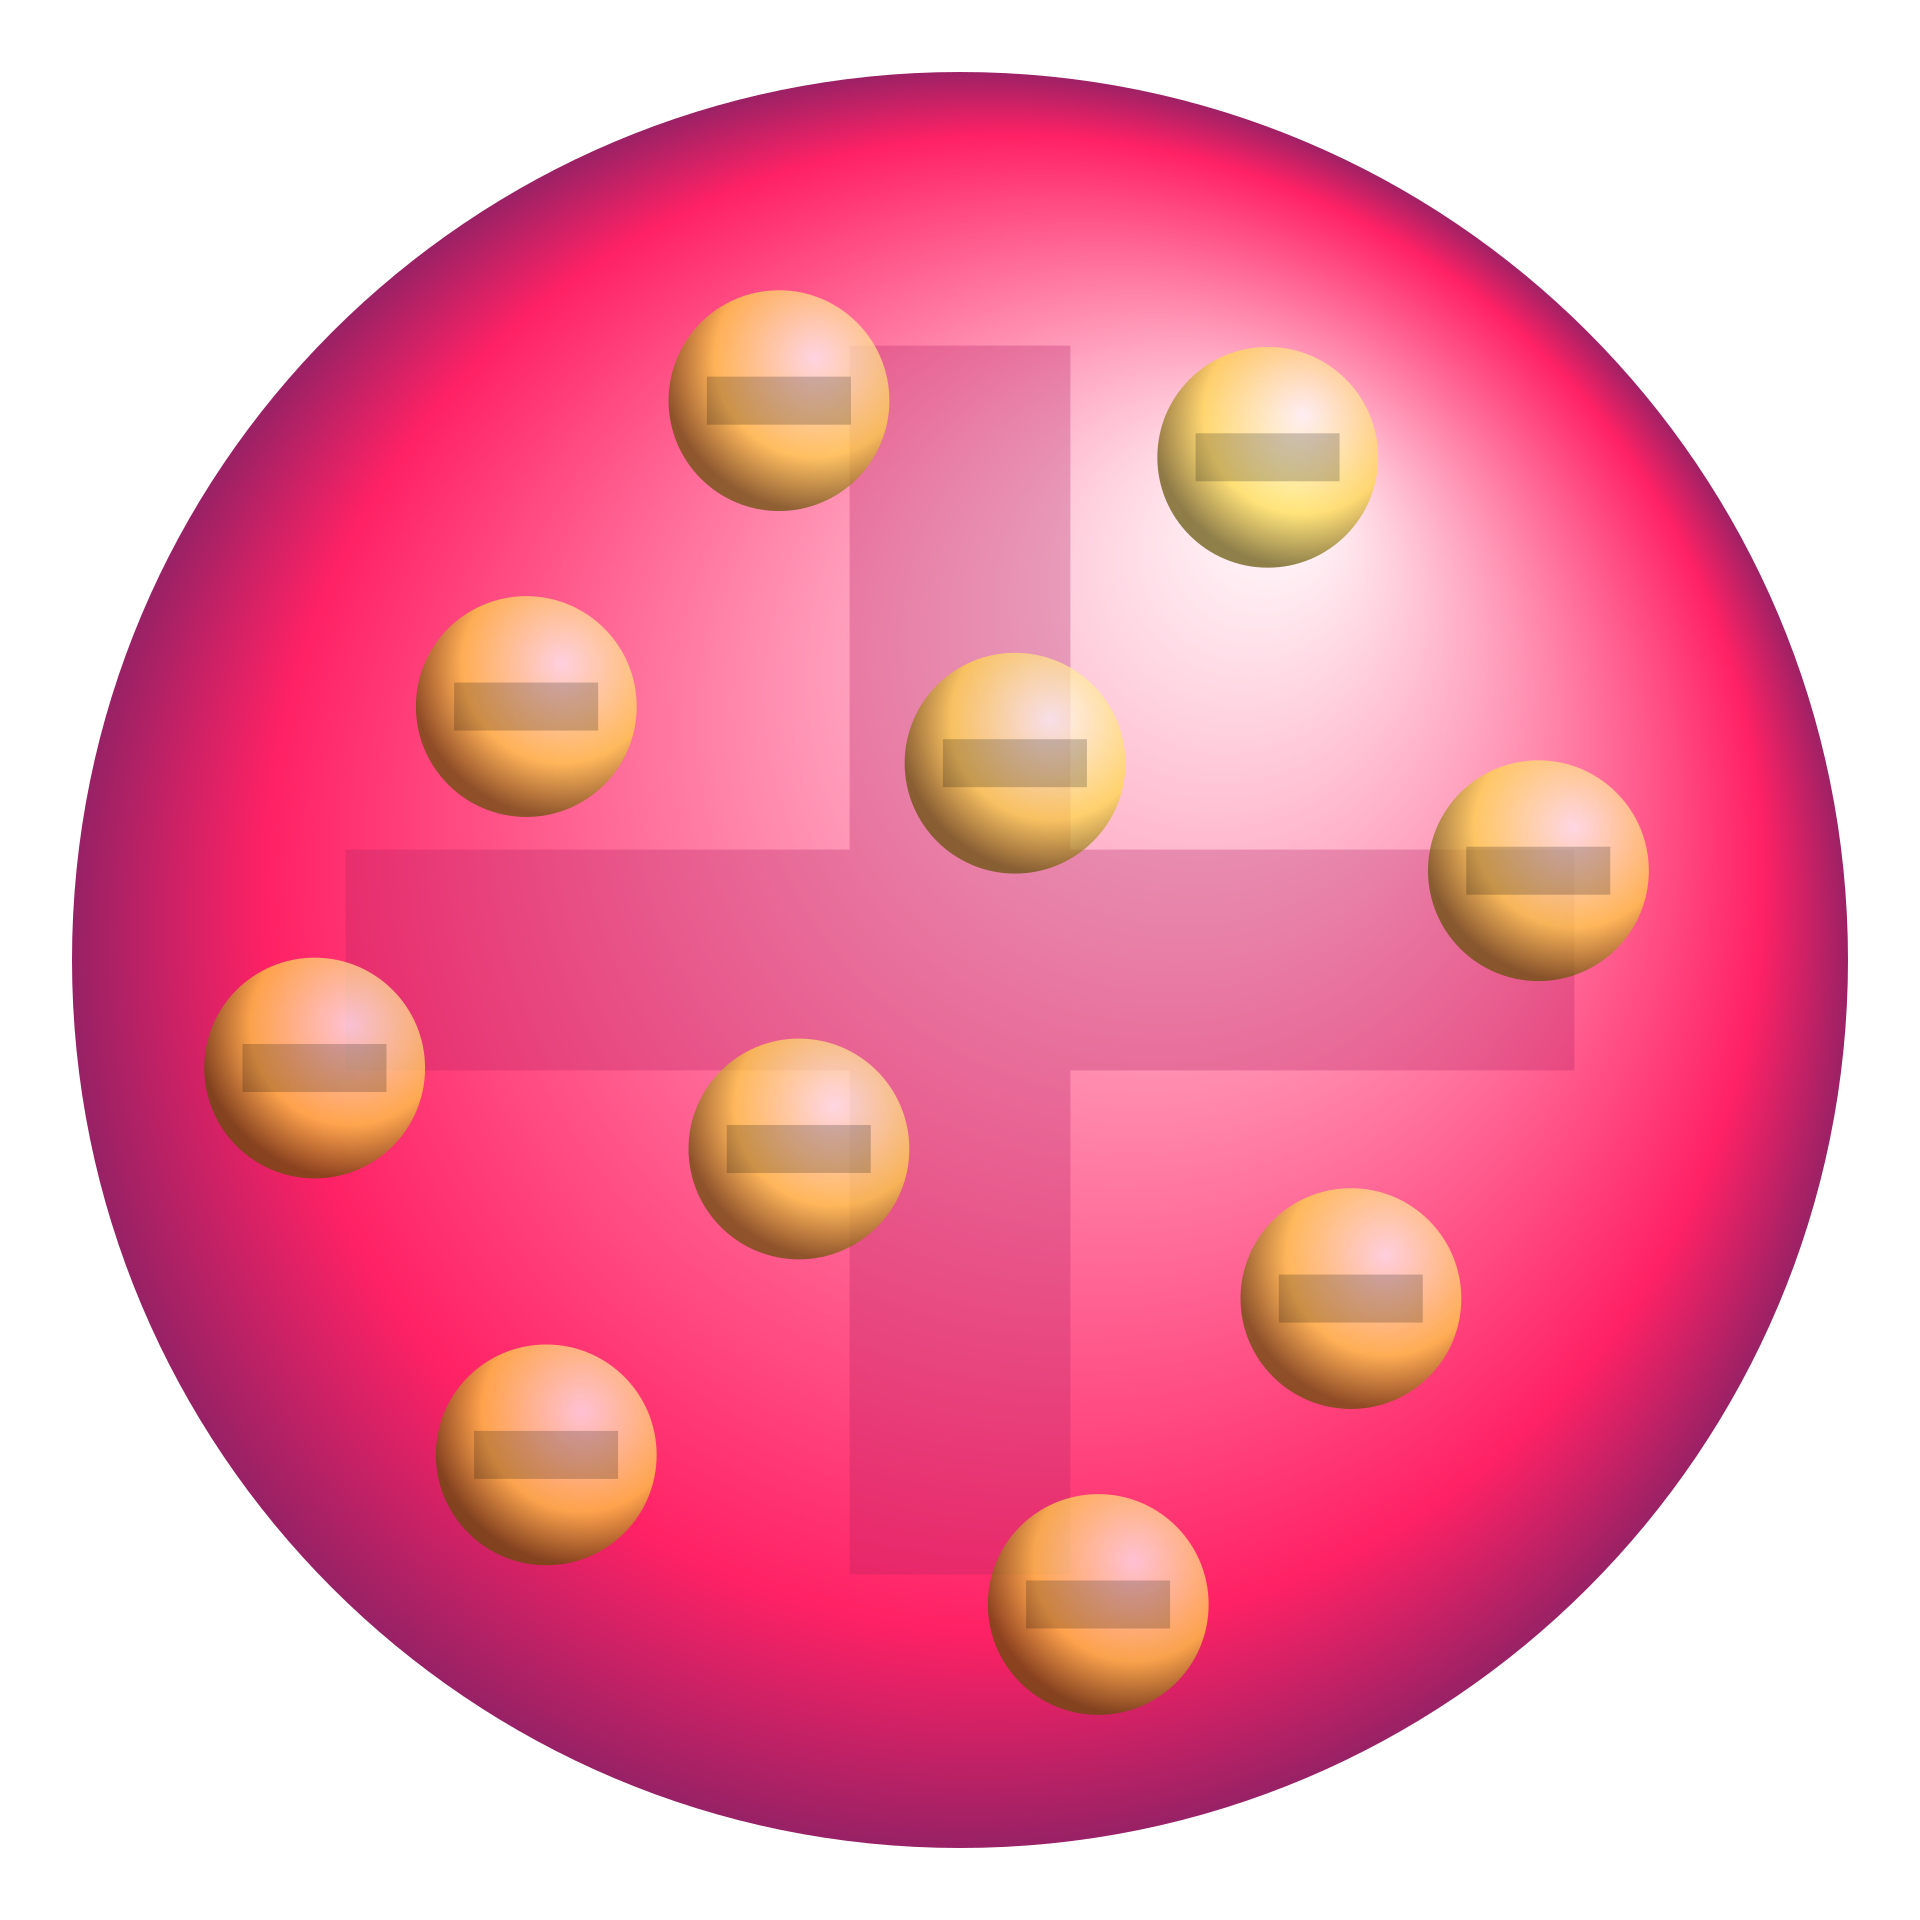
\includegraphics[width=10em]{./pictures/12.png}
                  \caption{枣糕结构}
              \end{minipage}
              \hfill
              \begin{minipage}{0.48\textwidth}
                  \centering
                  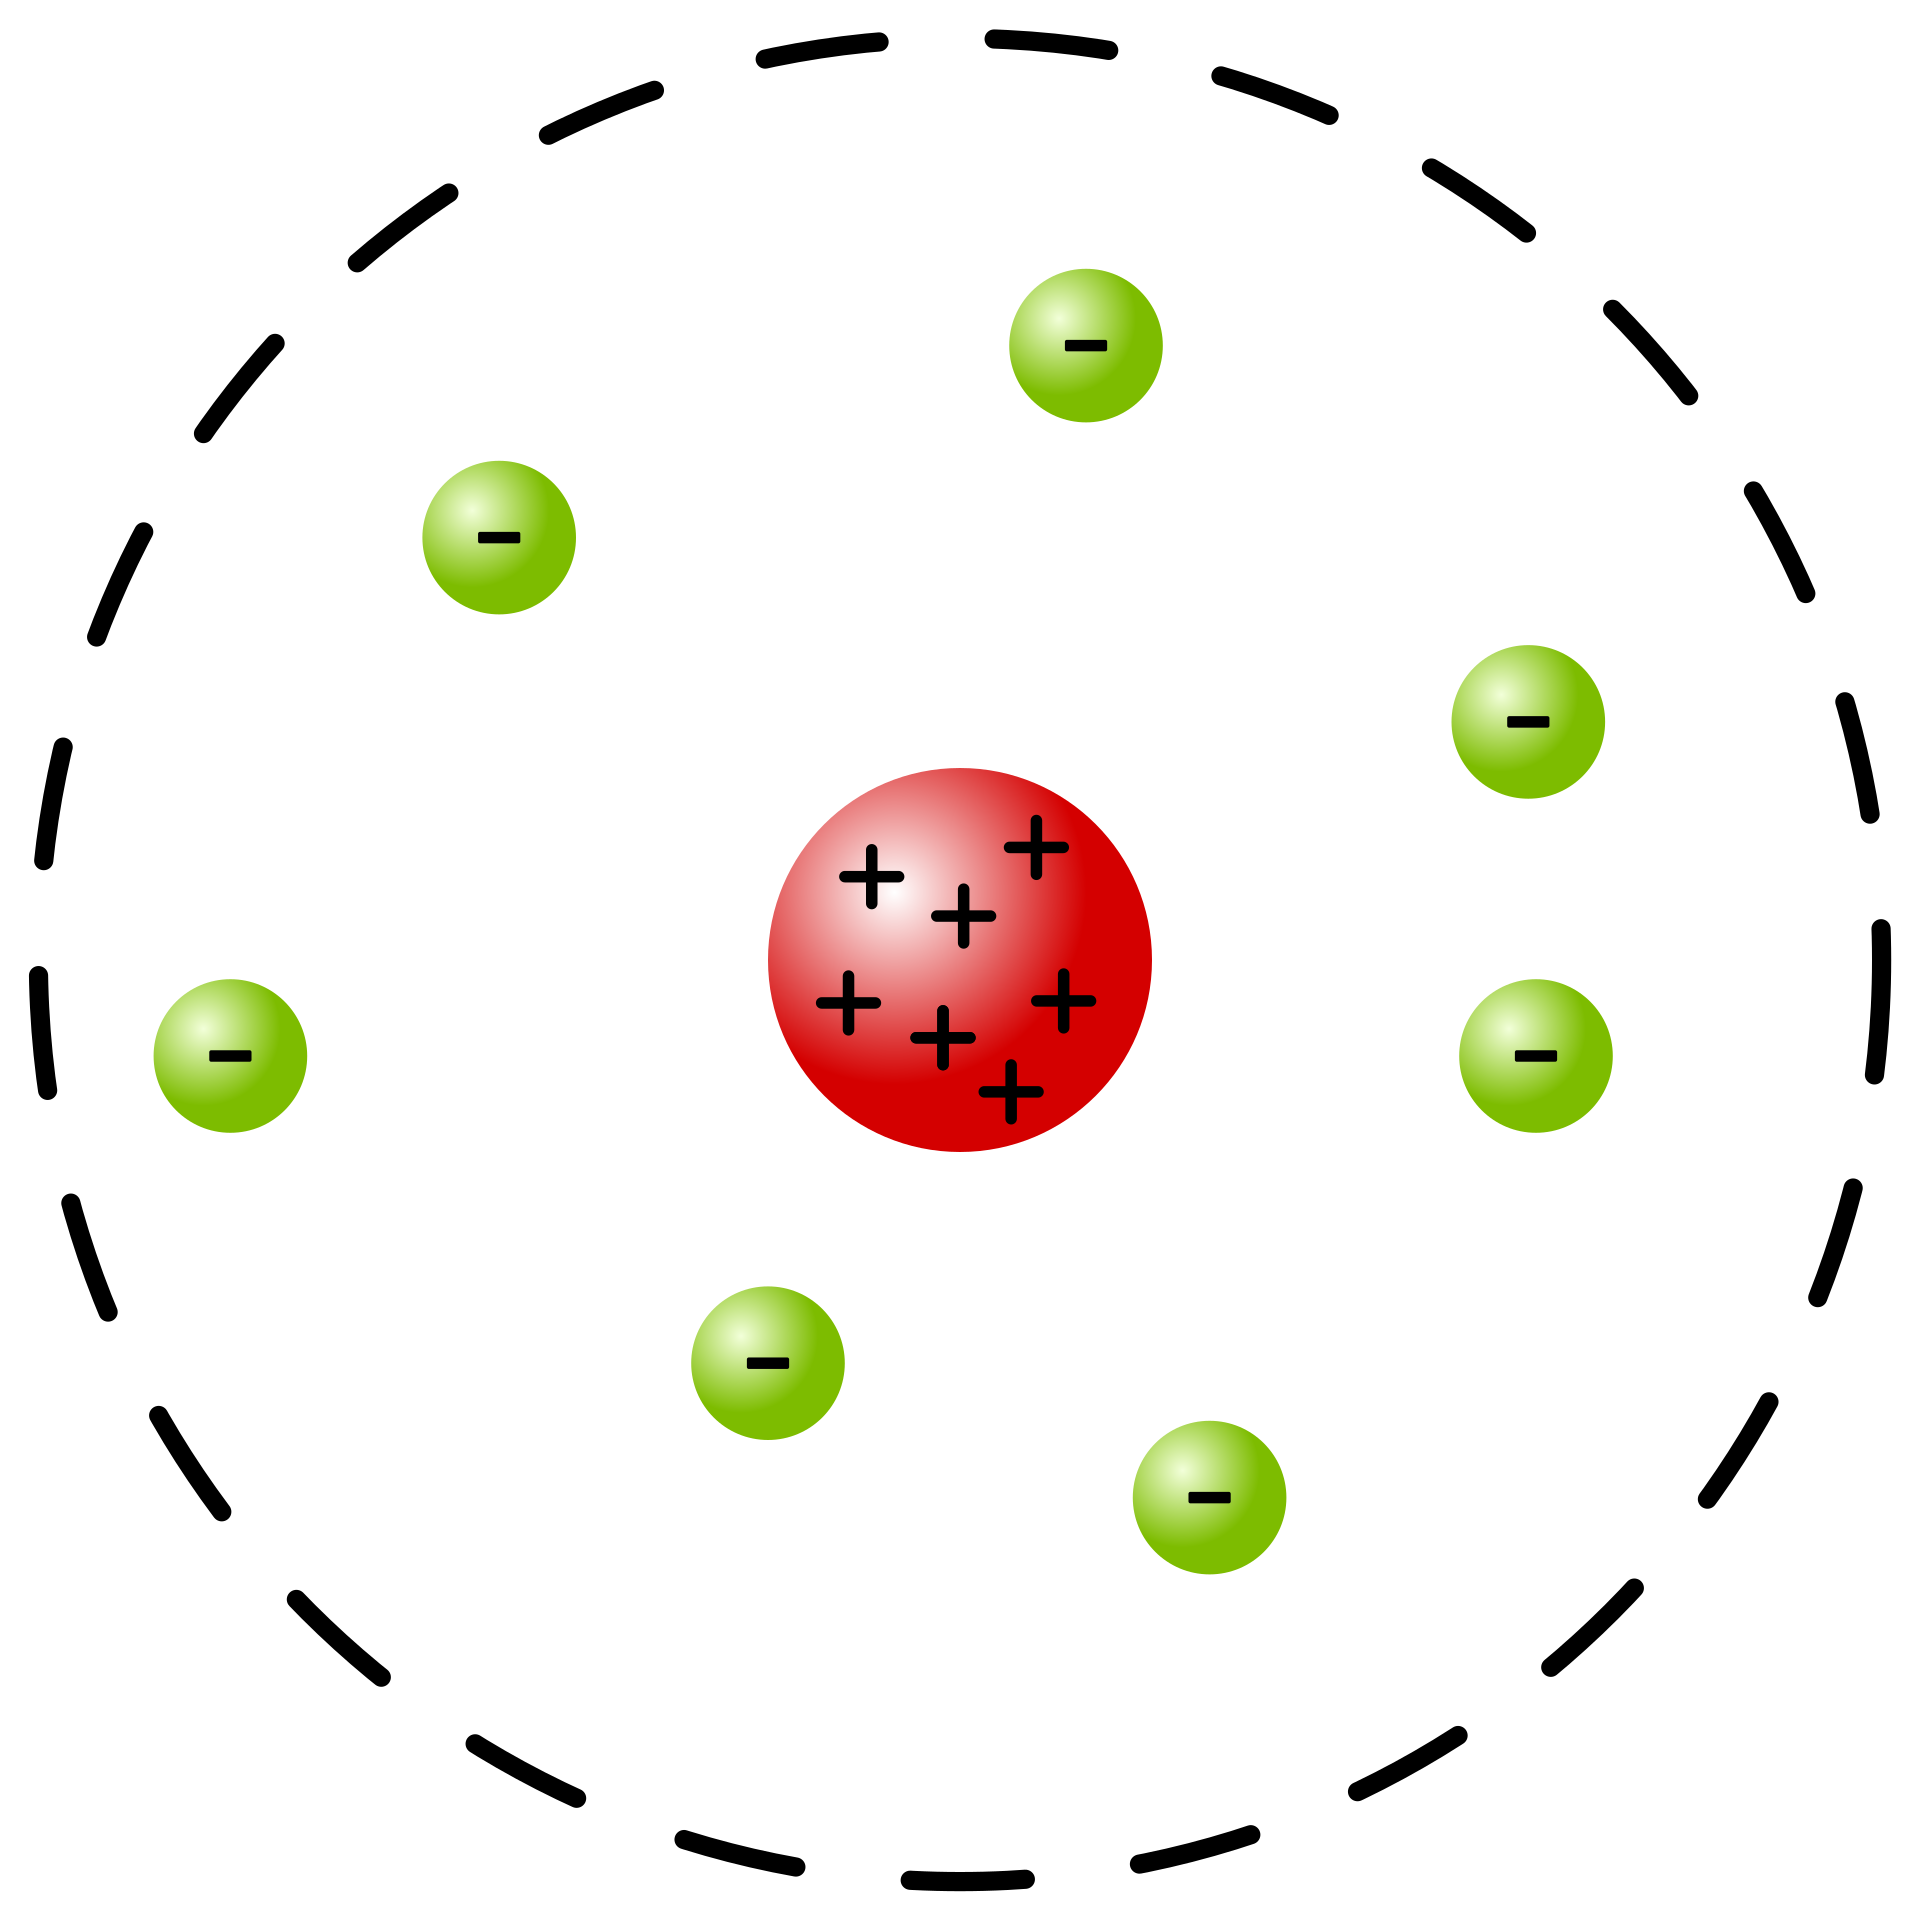
\includegraphics[width=10em]{./pictures/13.png}
                  \caption{核式结构}
              \end{minipage}
          \end{figure}
\end{enumerate}

\vspace{2em}

\subsubsection{\texorpdfstring{$\alpha$}*散射实验}
\begin{itemize}
    \item $\alpha$粒子: $He$原子核
    \item 实验原理: 使用$\alpha$粒子轰击金箔(原子间缝隙),边旋转荧光屏边接收粒子发光
    \item 实验中: 电子间的相互作用,质量,空气阻力等(极小);为何使用金箔(重,不易被碰撞影响;延展性好,可以做很薄)
    \item 实验结果
          \begin{itemize}
              \item[] 当时理论: 几乎所有粒子均可以穿过金箔
              \item[] 真实结果: 大部分穿过,少部分偏角较大,\textbf{极少部分反弹}(不符合枣糕结构模型)
              \item[] 结论: 原子内部极度空旷, 极少反弹现象是由集中的大量正电荷带来的库伦力造成
          \end{itemize}
\end{itemize}

\begin{center}
    \begin{figure}[h]
        \centering
        \begin{minipage}{0.58\textwidth}
            \centering
            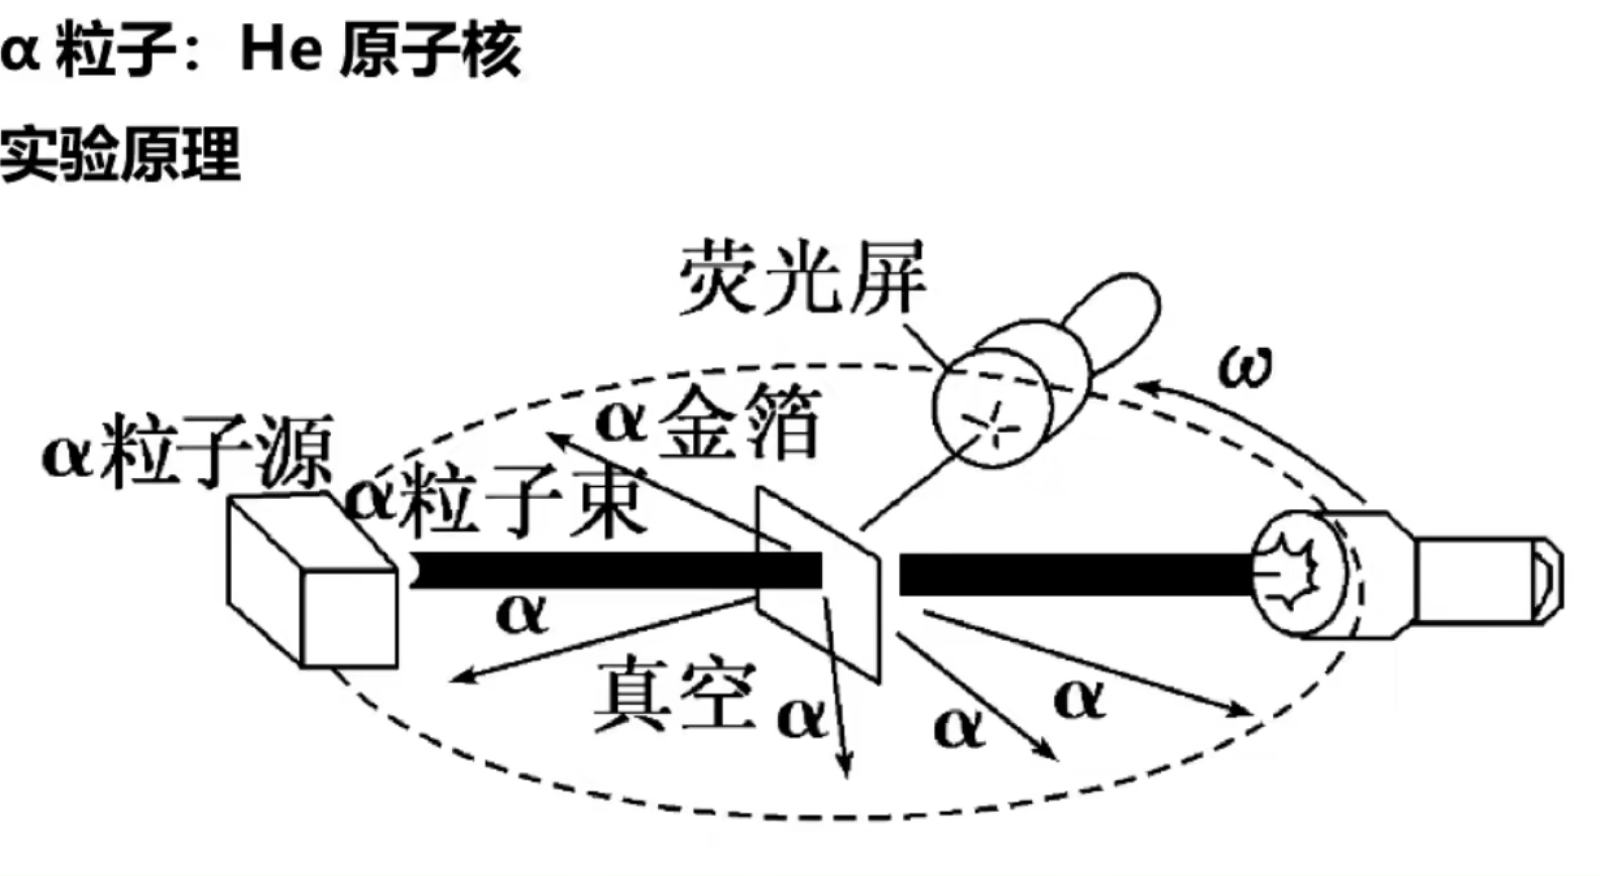
\includegraphics[width=25em]{./pictures/14.png}
        \end{minipage}
        \hfill
        \begin{minipage}{0.4\textwidth}
            \centering
            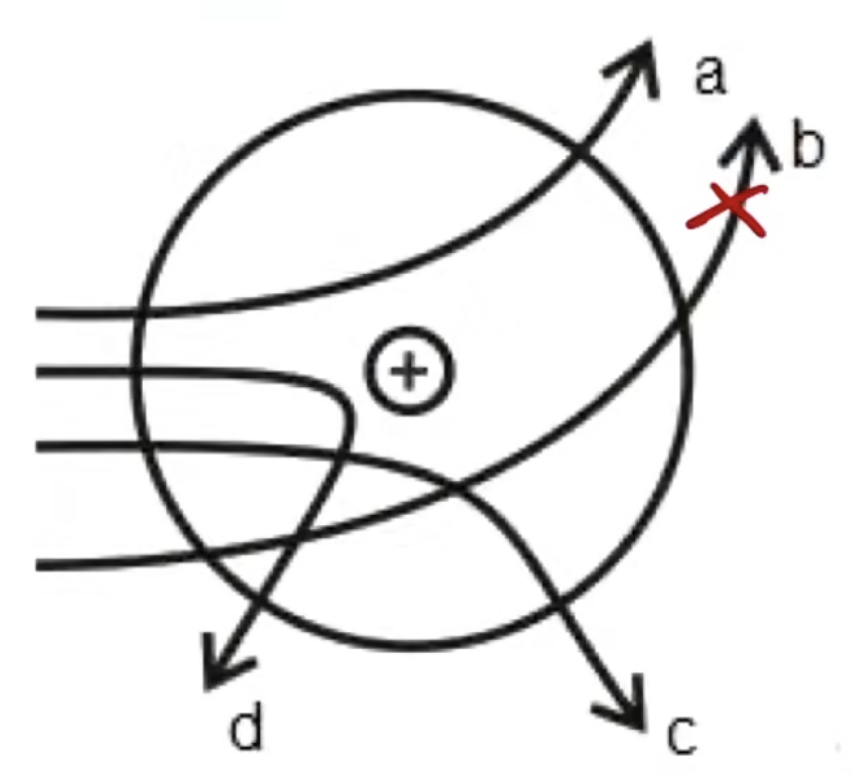
\includegraphics[width=16em]{./pictures/15.png}
        \end{minipage}
    \end{figure}
\end{center}

\vspace{2em}

\subsubsection{玻尔模型}
\begin{itemize}
    \item 经典理论的困难:
          \begin{itemize}
              \item 卢瑟福的核式结构正确指出了原子核的存在,很好的解释了$\alpha$散射实验,但是经典物理学
                    既无法解释原子的\textbf{稳定性},又无法解释原子\textbf{光谱的分立特性}.
              \item 绕核转动的电子在做周期性运动,其电磁场周期性的变化(波的传播)因而会激发电磁波,其绕核转动的能量将以电磁波的形式辐射出去.
                    所以电子绕核转动这个系统是不稳定的.然而事实是,原子是个很稳定的系统.
              \item 经典电磁理论,电子辐射的电磁波的频率就是其绕核转动频率.电子越转能量越小,那么离原子核就越来越近,转的也就越来越快,
                    这个变化应当是连续的,即应当是原子辐射各个频率的光都有(光谱应当是连续的).事实是分立的线状谱.
          \end{itemize}

          \begin{center}
              \begin{figure}[h]
                  \begin{minipage}{0.45\textwidth}
                      \centering
                      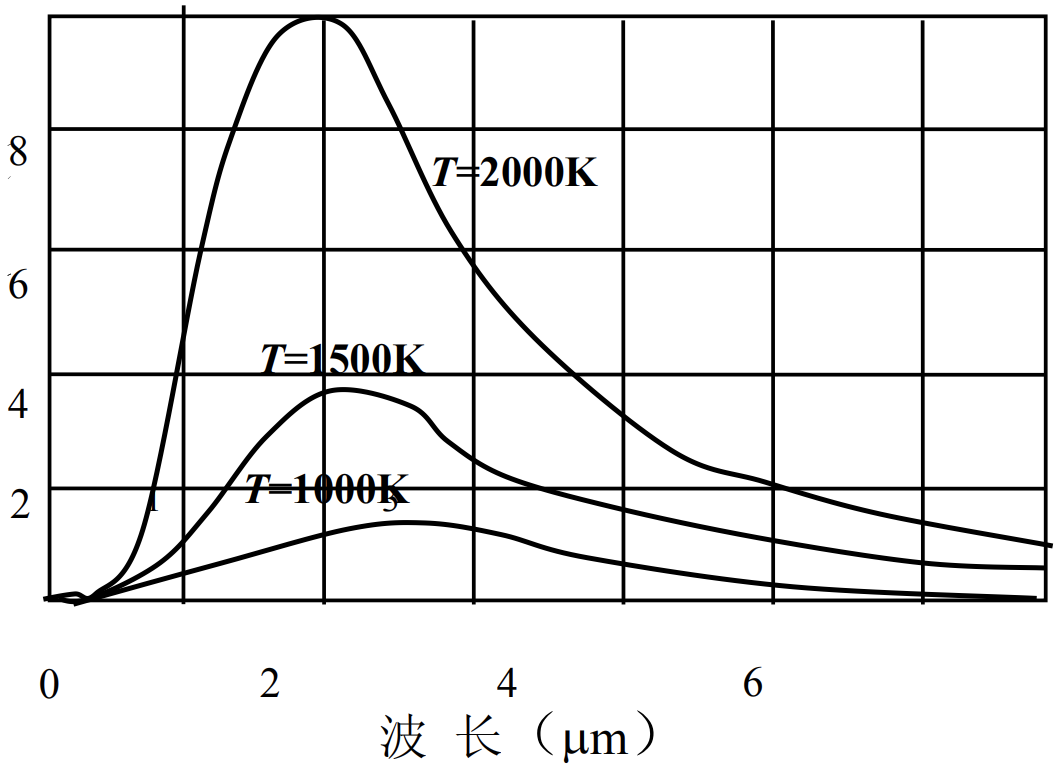
\includegraphics[width=\textwidth]{./pictures/16.png}
                      \caption*{Figure 1: 黑体辐射光谱}
                  \end{minipage}
                  \hfill
                  \begin{minipage}{0.5\textwidth}
                      \centering
                      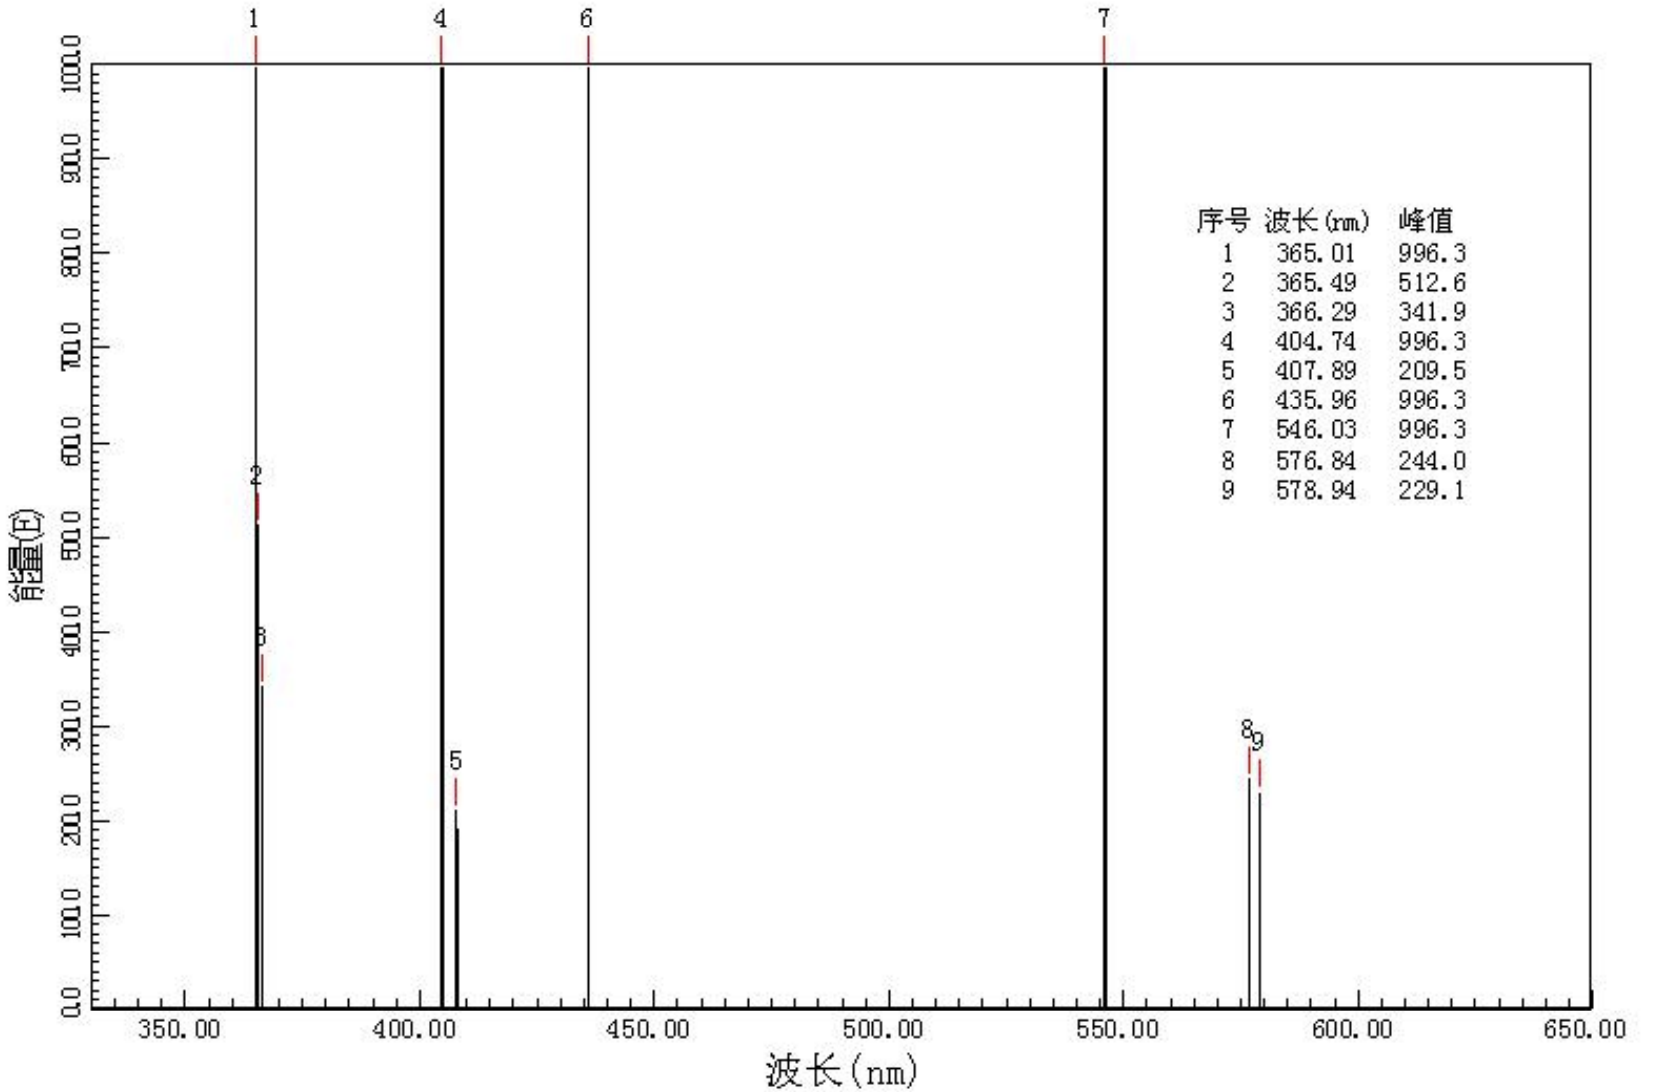
\includegraphics[width=\textwidth]{./pictures/17.png}
                      \caption*{Figure 2: 汞灯光谱}
                  \end{minipage}
              \end{figure}
          \end{center}
    \item 基本假设:
          \begin{itemize}
              \item[] 轨道量子化
              \item[]
                  \begin{minipage}{0.4\textwidth}
                      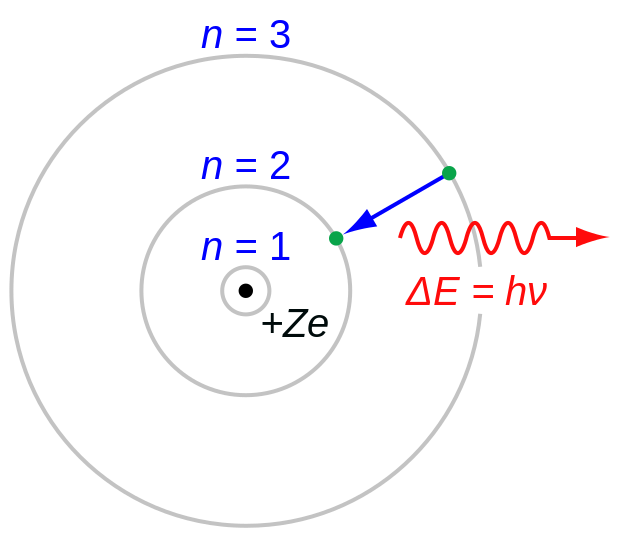
\includegraphics[width = \textwidth]{./pictures/18.png}
                  \end{minipage}
                  \hfill\hspace{-3em}
                  \begin{minipage}{0.52\textwidth}
                      \begin{itemize}
                          \item 电子\textbf{跃迁}辐射电磁波,电子在不同轨道运动$\llra$原子处于不同状态(原子跃迁)
                          \item 原子在不同的状态中具有不同的能量,因此原子的能量是\textbf{量子化},这些量子化的能量叫做\textbf{能级}
                          \item 原子中具有确定能量的稳定状态称为\textbf{定态}
                          \item 能量最低的态叫做\text{基态}$ n = 1 $;\textbf{激发态}$ n > 1 $(第一激发态$ n = 2 $)
                          \item[]
                              $\text{状态标识} \quad n = 1, \, 2, \, 3 \cdots$

                              $\text{能量标识} \quad E_{1}, \, E_{2}, \, E_{3}, \cdots$
                      \end{itemize}
                  \end{minipage}
                  \vspace{3em}
              \item[] 氢原子能级(以能级差示意跃迁难度)
              \item[]
                  \begin{minipage}{0.4\textwidth}
                      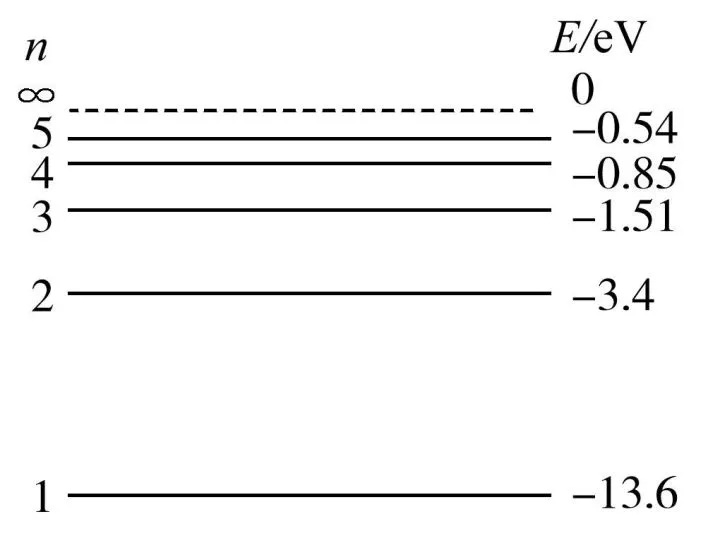
\includegraphics[width = \textwidth]{./pictures/19.png}
                  \end{minipage}
                  \hfill\hspace{-3em}
                  \begin{minipage}{0.52\textwidth}
                      \begin{itemize}
                          \item $E_{1}=-13.6eV \,\, E_{2} = -3.6eV \,\, E_{3} = -1.51eV $
                                $$E_{n} =  \dfrac{E_{1}}{n^{2}}$$
                          \item 电子吸收能量的方式:
                                \begin{itemize}
                                    \item[] \textbf{恰好}拥有某两能级差的光子(区别于光电效应中对光能量吸收的要求)
                                    \item[] \text{大于}某两能级差的实物粒子撞击
                                \end{itemize}
                          \item 电离: 电子吸收能量完全逃离(最远处能级为$0$)原子核的束缚
                      \end{itemize}
                  \end{minipage}
          \end{itemize}
    \item 电子跃迁(从高$\ra$低)
          \begin{itemize}
              \item 处于激发态的电子是不稳定的,将会\textbf{自发}从高能级向低能级跃迁
              \item 向低能级跃迁过程中会发射\textbf{特定频率}的电磁波(光)
              \item 有多种向低能级跃迁的方法时,跃迁结果不定,直至跃迁到基态
              \item 大量处于同一激发态的电子,所能发射电磁波的频率的种类最多$C_{n}^{2} = \frac{n(n-1)}{2}$
          \end{itemize}
\end{itemize}

\vspace{2em}

\subsection{天然放射性现象}
\begin{itemize}
    \item 定义: 放射性元素\textbf{原子核内部自发}放出射线的现象
    \item 三种射线:
          \begin{itemize}
              \item[] $\alpha$射线: $^{2}_{4}He$原子核 \, 速度$0.1c$
              \item[] $\beta$射线: $^{-1}_{0}e$ \, 速度$0.99c$
              \item[] $\gamma$射线: $^{0}_{0}n$电磁波 \, 速度$c$
              \item[] 电离能力: 使得被射线辐射的物质发生电离的能力 $\alpha > \beta > \gamma$

                  \vspace{-1em}
                  \begin{adjustbox}{minipage=0.91\linewidth, bgcolor=gray!20, padding=1em}
                      \small
                      距离足够近,放射性同位素释放出的$\alpha$粒子就足以穿透皮肤从而杀死皮下的重要组织的细胞.
                      相比$\gamma$射线和$x$光对细胞造成毁伤的能力,$\alpha$射线对细胞所造成的损坏程度超过其二十倍以上
                  \end{adjustbox}
                  \vspace{-1em}

              \item[] 穿透能力: 穿透物质能力 $\gamma > \beta > \alpha$ \, (甚至不能穿透一张纸)
              \item[] 磁场半径: $ r = \dfrac{mv}{qB} \quad q_{\alpha} = 2 q_{\beta}
                      \quad m_{\alpha} \gg m_{\beta} \lra r_{\alpha} > r_{\beta} $
              \item[] 电场偏转: $ a = \dfrac{Eq}{m} \quad q_{\alpha} = 2 q_{\beta}
                      \quad m_{\alpha} \gg m_{\beta} \quad a_{\alpha} < a_{\beta} $

                  \vspace{-1em}
                  \begin{adjustbox}{minipage=0.4\linewidth, bgcolor=gray!20, padding=1em}
                      \small
                      $\beta$粒子相比$\alpha$粒子在电磁场中更易发生偏转
                  \end{adjustbox}
                  \vspace{-1em}
          \end{itemize}
\end{itemize}

\vspace{2em}

\subsection{放射性元素的衰变}
\begin{enumerate}
    \item 原子核的表示: $_{Z}^{A}X$ \quad ($A$表质量数,$Z$为原子核的电荷数 \, eg. $_{4}^{2}He$)

          \vspace{-1em}
          \begin{adjustbox}{minipage=0.32\linewidth, bgcolor=gray!20, padding=1em}
              \small
              同位素: \, 质子数一样,质量数不一样
          \end{adjustbox}
          \vspace{-1em}

    \item 衰变形式:
          \begin{itemize}
              \item[] $\alpha$衰变: 放射性元素原子核放出$\alpha$粒子
                  $$
                      \nuc{238}{92}{U} \xlongrightarrow{\quad\quad} \nuc{234}{90}{Th}  + \nuc{4}{2}{He}
                  $$
              \item[] $\beta$衰变: 放射性元素原子核放出$\beta$粒子
                  $$
                      \nuc{234}{90}{Th} \xlongrightarrow{\quad\quad}  \nuc{234}{91}{Pa}+ \nuc{0}{-1}{e}
                  $$
          \end{itemize}
\end{enumerate}






\end{document}